\documentclass[../Thesis.tex]{subfiles}
\graphicspath{{\subfix{../figures/}}}
% \epstopdfsetup{outdir={../figures/}}
% \usepackage{xr}
% \externaldocument{C4 Method}
% \externaldocument{../_BackMatter/Appendix1}
\begin{document}

\chapter{Results and Discussion}\label{chap:results}
\textcolor{red}{An introduction to what is going to be included in this section. What results etc.}

In this section, we will investigate how the algorithms \autoref{alg:Gobs1} and \autoref{alg:ND} works in junction and individually. We shall observe how the algorithms can fail and what may be done to correct such cases.

\textcolor{red}{Overordnet pointe er at genere forskellige mulige graphisce modeller, som senere ville kunne bruges til at lave PGM el.l. Er nok bedst som et ekspolartivt værktøj, og vi undersøger her forskellige situationer, og hvornår der kan ske fejl ud fra om det er lange kæder af kausalitet eller mere komplekse strukturer}

% Initially, a few simple examples involving exponentiated multivariate Gaussians $\boldsymbol Y $.


\newpage
\section{Gaussian chains}\label{sec:Gaussian chains general}
In this section we discuss the errors made from the assumption that indirect effects can be computed as a sum of powers of the direct effects, i.e. $G_{indir} = \sum_{k\geq 1} G_{dir}^k$. In particular, on a theoretical level, we shall observe the error in $G_{obs}$ based on the above assumption of how similarities are \textit{convolved} which we equate with the noise $N$ from \autoref{subseq:Robustness to noise}, although it is a systematic error. To do this, we shall in this section use a multivariate Gaussian to be able to control the correlation and as an extension of this, the mutual information between pairs of random variables. As we already know, correlation and mutual information is independent of the mean and variance of each of the variables however for a bivariate Gaussian the mutual information is given by the correlation as stated in the following proposition.
\begin{proposition}\label{prop:MI bivariate gaussian}
    Given a bivariate normal distribution $\boldsymbol X \sim \mathcal{N}\left(\boldsymbol \mu,  \Sigma\right)$ where
    $$\Sigma =
        \begin{bmatrix}
            \sigma_1^2             & \rho \sigma_1 \sigma^2 \\
            \rho \sigma_1 \sigma_2 & \sigma_2^2
        \end{bmatrix}
    $$
    Then the mutual information $I\left(X_1, X_2\right) = -\frac{1}{2}\ln \left(1 - \rho^2\right)$.
\end{proposition}
\begin{proof}
    This follows by direct computation Using e.g. that $I(X_1, X_2) = h(X_1) + h(X_2) - h(X_1, X_2)$
\end{proof}
Thus, if we know a correlation structure of a Gaussian random vector, we also know the mutual information between every pair of variables which we shall now use in the following made up example. Namely, what we shall denote as a Gaussian chain defined as a Gaussian random vector in the following way. Let $\boldsymbol X$ be a $d$-dimensional Gaussian random vector, the $\boldsymbol X$ is a standard Gaussian chain if it can be written in the following way in terms of $d$ independent standard normal variables $Z_i$ up to a permutation i.e. there exists a permutation of the variables of the random vector $\boldsymbol X$ that permits the following structure.
\begin{equation}\label{eq:Gaussian chain def}
    \begin{split}
        X_1 & = Z_1                                                                  \\
        X_2 & = \vec{\rho}_{1,2} X_1 + \sqrt{1 - \vec{\rho}_{1,2}^2} Z_2             \\
        X_3 & = \vec{\rho}_{2,3} X_2 + \sqrt{1 - \vec{\rho}_{2,3}^2} Z_3             \\
            & \vdots                                                                 \\
        X_d & = \vec{\rho}_{d-1, d} X_{d-1} + \sqrt{1 - \vec{\rho}_{d-1, d}^2} Z_{d}
    \end{split}
\end{equation}
It follows that the marginals have variance $1$ as clearly $\text{Var} \left[X_1\right] = \text{Var}\left[Z_1\right] = 1$ and for $i > 1$, $\text{Var}\left[X_i\right] = \vec{\rho}_{i-1,i}^2 \text{Var}\left[X_{i-1}\right] + \left(1 - \vec{\rho}_{i-1,i}^2\right) \text{Var} \left[Z_i\right] = 1$ by independence of $X_{i-1}$ and $Z_i$. Thus, the above structure also implies the Cholesky factorization of the correlation matrix for $\boldsymbol X$, namely
$$L = \begin{bmatrix}
        1                                &                                               &                                                                    &        &                                \\
        \vec{\rho}_{1,2}                 & \sqrt{1 - \vec{\rho}_{1,2}^2}                 &                                                                    &        &                                \\
        \vec{\rho}_{2,3}\vec{\rho}_{1,2} & \vec{\rho}_{2,3}\sqrt{1 - \vec{\rho}_{1,2}^2} & \sqrt{1 - \vec{\rho}_{2,3}^2}                                      &        &                                \\
        \vdots                           &                                               &                                                                    & \ddots &                                \\
        \prod_{i=2}^d \vec{\rho}_{i-1,i} & \dots                                         & \sqrt{1 - \vec{\rho}_{j-1,j}^2} \prod_{i=j+1}^d \vec{\rho}_{i-1,i} & \dots  & \sqrt{1- \vec{\rho}_{d-1,d}^2}
    \end{bmatrix}$$
Which will allow us to both sample from such a chain and calculate $G_{dir}$ and $G_{obs}$ theoretically. However, in this example, it is easier to calculate the correlation between the variable $X_i$ and $X_j$ directly. As the variance of each variable is $1$ we simply calculate the covariance. We assume without loss of generality that $i < j$ whence
$$\text{Cov}\left[X_i, X_j\right] = \text{Cov}\left[X_i, \vec{\rho}_{j-1,j} X_{j-1} + \sqrt{1 - \vec{\rho}_{j-1,j}^2}Z_j\right] = \vec{\rho}_{j-1,j} \text{Cov}\left[X_i, X_{j-1}\right]$$
which by induction implies $\rho_{i,j} = \prod_{k=i+1}^{j} \vec{\rho}_{k-1,k} = \rho_{j,i}$. At this point, we are almost ready to use the algorithms from the previous chapter. First, we will only use \autoref{alg:ND} to deconvolve the network based on theoretical correlations and later mutual information. However, before doing so, we note that from the definition in \autoref{eq:Gaussian chain def} the random variable $\boldsymbol X$ exhibits a Markovian property. Namely, the $X_i$ above can be understood discrete stochastic process as they are successively drawn based only on the previous variable $X_{i-1}$ i.e. $f\left(x_i \mid X_{i-1}, X_{i-2} , \dots , X_{1}\right) = f\left(x_i \mid X_{i-1}\right)$. Thus, if the algorithm works as intended, we should observe that the deconvolved network is a \textit{chain} of variables as shown in the \autoref{fig:gaussian chain expected res}
\begin{figure}[ht]
    \centering
    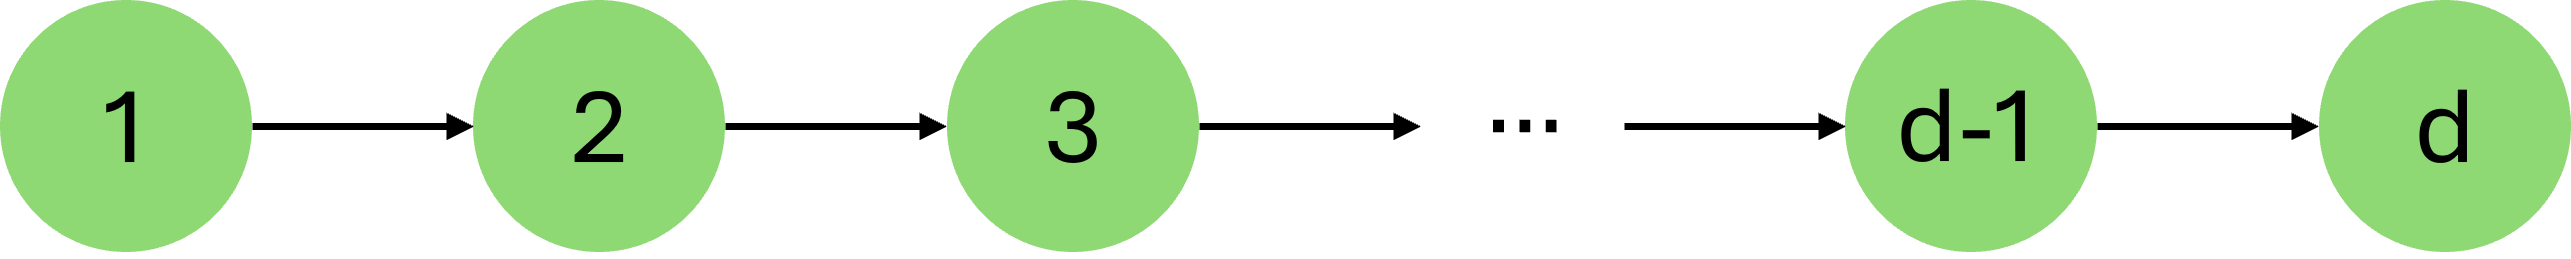
\includegraphics[width = .7\linewidth]{figures/ND examples/Gaussian chain.png}
    \caption{The graphical representation of a Gaussian chain. Arrows signify a possible causal structure. If furthermore, one assumes that $X_1$ is generated first, then $X_2$ and so on, this is the only causal structure that would make sense.}
    \label{fig:gaussian chain expected res}
\end{figure}
Thus, we now have the expected result, and we proceed with using correlation and mutual information to try and rediscover this structure in the following two sections

\subsection{Gaussian chain deconvolution using correlation}
In this section, we will use the observed correlations as elements of $G_{obs}$. In particular, the $(i,j)$ entry of $G_{obs}$ is $\rho_{i,j} = \prod_{k=i+1}^{j} \vec{\rho}_{k-1,k}$ when $i< j$ and $0$ otherwise. This makes $G_{obs}$ strictly upper triangular. Note that although it makes sense to consider the correlation between a variable and itself, we shall as discussed before set the diagonal to $0$. The reason for this becomes clear when we try to convolve $G_{dir}$ based on the initial definition of a general Gaussian chain in \autoref{eq:Gaussian chain def}. We note that in \autoref{alg:Gobs1} we usually (without an assumption of the topology of the random variables) use a symmetrical $G_{obs}$. We shall however postpone this discussion a bit and first use an upper triangular $G_{obs}$. In particular, we shall observe that we perfectly recover the \textit{directional} correlations $\vec{\rho}_{k-1,k}$ from \autoref{eq:Gaussian chain def} through \autoref{eq:Gdir from Gobs}.

As $G_{obs}$ is in this case strictly upper triangular, the spectral radius is $0$ and hence we have no problems with convergence of the infinite sum of powers of (the uniquely defined) $G_{dir}$. From the above, it is clear that $G_{obs}$ is given as follows
\begin{equation}\label{eq:Gaussian chain G_obs triangular form}
    G_{obs} = \begin{bmatrix}
        0 & \vec{\rho}_{1,2} & \vec{\rho}_{1,2}\,\vec{\rho}_{2,3} & \dots & \prod_{k=2}^{d} \vec{\rho}_{k-1,k} \\
          & 0                & \vec{\rho}_{2,3}                   & \dots & \prod_{k=3}^{d} \vec{\rho}_{k-1,k} \\
          &                  & \ddots                             &       & \vdots                             \\
          &                  &                                    & 0     & \vec{\rho}_{d-1,d}                 \\
          &                  &                                    &       & 0
    \end{bmatrix}
\end{equation}
Now, let $G_{dir}$ be given as follows
$$G_{dir} = \begin{bmatrix}
        0 & \vec{\rho}_{1,2} &                  &        &                    \\
          & 0                & \vec{\rho}_{2,3} &        &                    \\
          &                  & \ddots           & \ddots &                    \\
          &                  &                  & 0      & \vec{\rho}_{d-1,d} \\
          &                  &                  &        & 0
    \end{bmatrix}$$
then $G_{dir}^2$ is given by
$$G_{dir}^2 = \begin{bmatrix}
        0 & 0 & \vec{\rho}_{1,2}   \, \vec{\rho}_{2,3} &                                      &        &                                           \\
          & 0 & 0                                      & \vec{\rho}_{2,3} \, \vec{\rho}_{3,4} &        &                                           \\
          &   & \ddots                                 & \ddots                               & \ddots &                                           \\
          &   &                                        & 0                                    & 0      & \vec{\rho}_{d-2,d-1}\, \vec{\rho}_{d-1,d} \\
          &   &                                        &                                      & 0      & 0
    \end{bmatrix}$$
It is not hard to show that in fact $\sum_{k\geq 1} G_{dir}^k = \sum_{k=1}^d G_{dir}^k = G_{obs}$. Thus, if we know a graph topological ordering of the random variables corresponding to the structural causal model, we completely recover (without any error) the direct dependencies/correlation from to the initial definition in \autoref{eq:Gaussian chain def}. This result holds for a general \textit{chain} where $Z_i$ can follow any distribution as long as they are uncorrelated. This follows from the above computation of $\text{Cov}\left[X_i,X_j\right]$, where no assumption of $Z_j$ was needed except for correlation $0$.

From the above, we might think that if we have a topological ordering of the random variables this is the preferred method, and it is as long as correlation is a good enough measure of similarity/codependency. Albeit this is only shown for the special case of a chain, in \autoref{sec:General Gaussian graph} we consider the more general case and conclude that this indeed holds. Regarding the comment on correlation being a good enough measure of similarity, a prototypical case is when joint probability density function of two variables resemble a parabola. Namely, let $X_1\sim \mathcal{U}\left(0,1\right)$ and $X_2 \mid X_1 \sim \mathcal{N}\left(1 - 4\left(x_1 - 1/2\right)^2 , \sigma^2\right)$ i.e. $X_2 = 1 - 4 \left(X_1 - 1/2\right)^2 + \epsilon$ where $\epsilon \sim \mathcal{N}\left(0,\sigma^2\right)$. In \autoref{fig:MI parabola example}, $1000$ samples from this distribution is shown for $\sigma = 1/10$ along with the expectation $\mathbb{E}\left[X_2 | X_1\right]$. It is not hard to show that the covariance between $X_1$ and $X_2$ is $0$ however we clearly see a relationship between the two variables. In fact, computing the mutual information results in $I\left(X_1,X_2\right) \approx 1.030$ implying $X_1 \not\perp X_2$ i.e. there exists a higher order (non-linear) dependency. Thus, if the algorithm permits, we would prefer mutual information to correlation as we can then use observed higher order relationships to infer a causal structure.
\begin{figure}[ht]
    \centering
    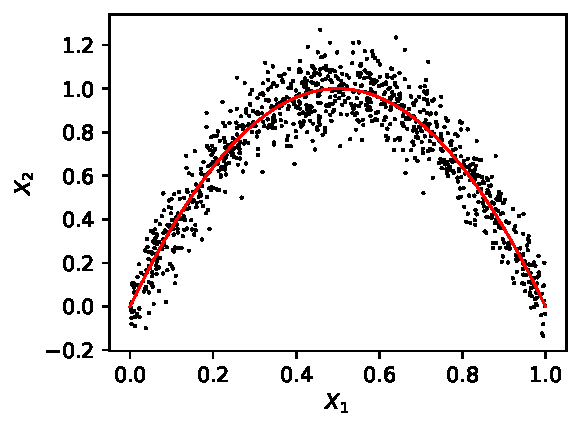
\includegraphics[width=.55\linewidth]{figures/Mutual information figures/parabola example.pdf}
    \caption{1000 samples generated from $X_1\sim \mathcal{U}\left(0,1\right)$ and $X_2 \mid X_1 \sim \mathcal{N}\left(1 - 4\left(x_1 - 1/2\right)^2 , \sigma^2\right)$ with $\sigma = 1/10$. The mutual information is calculated theoretically to be $I\left(X_1,X_2\right) \approx 1.030$ and repeated simulations show that the empirical correlation is symmetric around $0$ supporting the claim that the underlying correlation is in fact $0$} % 1.0296516475133333
    \label{fig:MI parabola example}
\end{figure}
On a more technical point of view, we note that mutual information is a measure of how dense the joint distribution is, invariant to scale. In a way, it is a measure of how close the joint distribution is to a lower dimensional manifold.

We proceed with a $10$-Gaussian chain defined by the following correlations:
\begin{equation}\label{eq:Example Gaussian chain}
    \begin{aligned}
        \rho_{1,2} & = 0.6, & \rho_{2,3} & = 0.5, & \rho_{3,4}  & = 0.4 \\
        \rho_{4,5} & = 0.2, & \rho_{5,6} & = 0.9, & \rho_{6,7}  & = 0.8 \\
        \rho_{7,8} & = 0.9, & \rho_{8,9} & = 0.8, & \rho_{9,10} & = 0.7
    \end{aligned}
\end{equation}
We have chosen correlations of different sizes to check if the deconvolution is robust in presence of both strong and weak links. In particular, $X_5$ is only $\rho_{4,5}^2 = 4\%$ of $X_4$ and the remaining $96\%$ is noise/indescribable variance i.e. a very weak link between the first part of the chain up to and including $X_4$ and the rest. However, as discussed above, if let $G_{obs}$ be upper triangular, we should completely rediscover these direct relations which is indeed also the case. In particular, from \autoref{fig:Gaussian chain triangular G_obs using correlation} we observe that the inferred network, represented by $G_{dir}$, is indeed a chain of variables and is exactly equal to the theoretical $G_{dir}$ as we would expect (up to very small rounding errors of the size $10^{-16}$). The \textit{estimated} $G_{dir}$ is also shown as a directed graph which the initial topological assumption implies, with edges wherever $G_{dir}$ is non-zero.
\begin{figure}[H]
    \centering
    \begin{subfigure}[t]{0.49\textwidth}
        \centering
        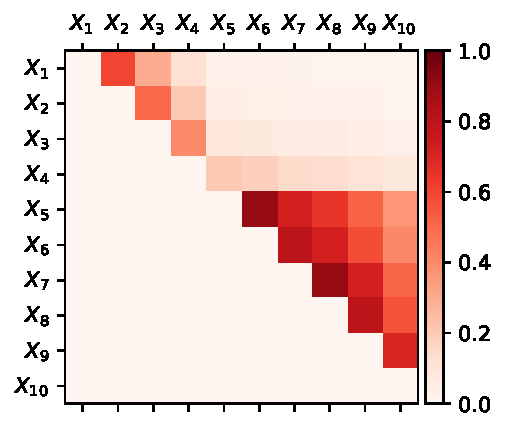
\includegraphics[width=.95\linewidth]{figures/Gaussian Chain Theoretical/triangular G obs.pdf}
        \caption{$G_{obs}$}
        % \label{fig:Gaussian 3x3 large s}
    \end{subfigure}
    \hfill
    \begin{subfigure}[t]{0.49\textwidth}
        \centering
        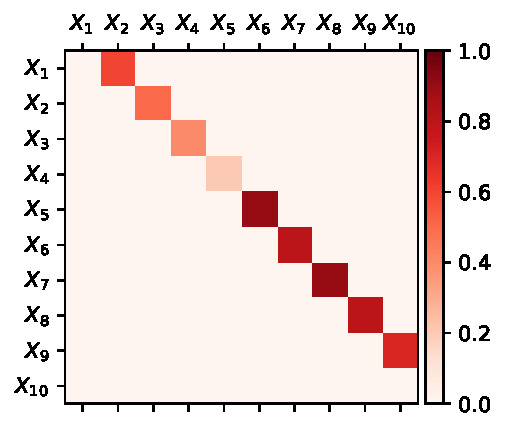
\includegraphics[width=.95\linewidth]{figures/Gaussian Chain Theoretical/G dir from triangular G obs.pdf}
        \caption{$G_{dir}$}
        \label{subfig:Gaussian chain triangular G_obs using correlation - G_dir}
    \end{subfigure}
    \\[\baselineskip]
    \begin{subfigure}[t]{0.49\textwidth}
        \centering
        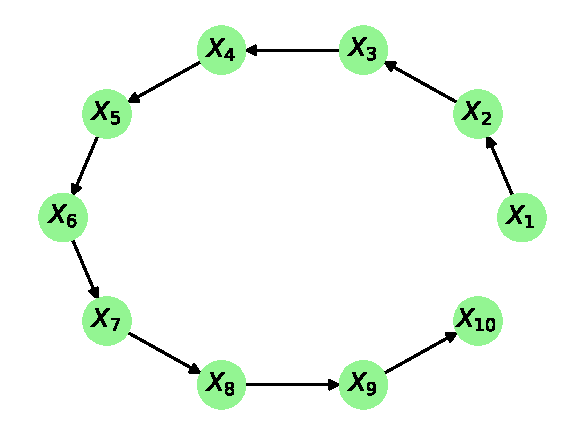
\includegraphics[width=.9\linewidth]{figures/Gaussian Chain Theoretical/Chain graph from triangular G obs.pdf}
        \caption{$G_{dir}$ as a digraph}
        % \label{fig:Gaussian 3x3 large s}
    \end{subfigure}
    \caption{Results from using an upper triangular $G_{obs}$ and correlation to infer the causal network structure. (a) shows the upper triangular $G_{obs}$ with the correlation between every pair of variables. (b) shows the deconvolved $G_{obs}$ and as we expect, the superdiagonal contains the original correlations given in \autoref{eq:Example Gaussian chain}. (c) shows $G_{dir}$ represented as a digraph and matches the expected result.}
    \label{fig:Gaussian chain triangular G_obs using correlation}
\end{figure}
We now proceed to investigate what happens when we remove the prior information of the topological ordering. Namely, if $G_{obs}$ is no longer triangular but symmetric. In particular, let $T_{dir}$ be given as $G_{dir}$ above. We then have that $G_{dir}$ in the symmetric case is $T_{dir} + T_{dir}^T$ and similarly for $G_{obs}$, $G_{obs} = T_{obs} + T_{obs}^T$. Clearly, $I + G_{obs}$ is positive definite as it is a proper correlation matrix. However, that also implies that we might have eigenvalues of $G_{obs}$ less than or equal to $-1/2$ which we know from \autoref{subsec:Setup and assumptions} is not the result of a $G_{dir}$ such that \autoref{eq:Gobs from Gdir} holds as then the infinite sum diverges. However, as $-1$ is not an eigenvalue of $G_{obs}$, we will investigate what happens if one tries to use \autoref{eq:Gdir from Gobs} anyway.

But first, we shall discuss the errors being made using the symmetric $G_{obs}$ and $G_{dir}$ instead of triangular. Namely, we investigate the powers of $G_{dir}$:
$$G_{dir}^2 = \left(T_{dir} + T_{dir}^T\right)^2 = T_{dir}^2 + \left(T_{dir}^T\right)^2 + T_{dir} T_{dir}^T + T_{dir}^T T_{dir}$$
Higher power can be calculated similarly, but for the second power we already observe an error. The first two terms corresponds to a reflection of the second order effects that we saw above and know to be true, whence the final two terms, that add to a diagonal matrix, is an error and will propagate with higher order powers of $G_{dir}$. Through simple calculation the resulting error is
$$T_{dir} T_{dir}^T + T_{dir}^T T_{dir} = \begin{bmatrix}
        \rho_{1,2}^2 + \rho_{2,3}^2 &                             &        &                                   \\
                                    & \rho_{2,3}^2 + \rho_{3,4}^2 &        &                                   \\
                                    &                             & \ddots &                                   \\
                                    &                             &        & \rho_{d-2,d-1}^2 + \rho_{d-1,d}^2
    \end{bmatrix}$$
Thus, for chains, we expect larger errors for sub-chains with strong links i.e. a subgraph of a chain that is also a chain where the correlation from one variable to the next is large. Using $G_{obs} = T_{obs} + T_{obs}^T$ we have that the smallest eigenvalue is approximately $\lambda_{\min} \approx -0.92263$ thus, multiplying $G_{obs}$ with a constant $c_s < 0.54192$ will make $G_{dir}$ have spectral radius at most $1$. The results vary with one or two edges for the choice of $c_s$ and in the following we have chosen $c_s = 0.53651$ resulting in $\rho\left(G_{dir}\right) \approx 0.98020$ and $\tilde{G}_{obs}$ and $\tilde{G}_{dir}$ as seen in \autoref{fig:Gaussian chain symmetric G_obs using correlation}. From \autoref{subfig:Gaussian chain symmetric G_obs using correlation - G_dir} we see that some correlation/association seem to bleed to variables $2$ or $3$ edges away which we of course know is not true given the Markov property discussed above. However, it is also clear that the error here is that the original assumption does not hold since using a symmetric $G_{obs}$ imply that the measure of similarity flows both ways where in this case it is very much unidirectional.

From \autoref{fig:Gaussian chain symmetric G_obs using correlation} conclude that we are somewhat able to rediscover the causal structure. Not surprisingly, we observe that the weak link between $X_4$ and $X_5$ is one of the first to break and that we observe some extra edges between the later more strongly linked sub-chain as by the above discussion. Finally, before presenting the results for the unscaled $G_{obs}$ (where the smallest eigenvalue is smaller than $-1/2$) we note that changing the parameter $\alpha$ in \autoref{alg:ND} did not have much of an effect indicating that the network is quite sparse (as we also know it to be) as even removing $65\%$ of the smallest correlations from $G_{obs}$ did not have any effect. The chosen threshold of $t=0.2$ on $G_{dir}$ seemed to be the best compromise of a connected graph and the density of the edges (although this is somewhat biased from prior knowledge of the true graphical structure).
% Also, trying to have $1$ in the diagonal instead of $0$ worsened the result
\begin{figure}[H]
    \centering
    \begin{subfigure}[t]{0.49\textwidth}
        \centering
        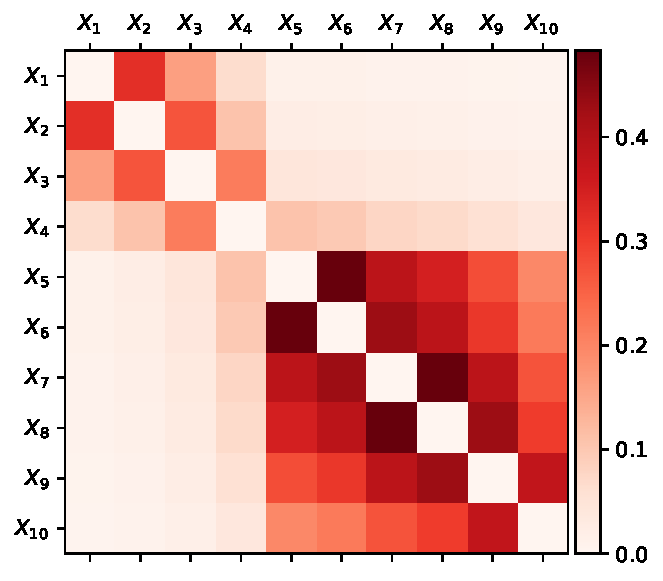
\includegraphics[width=.95\linewidth]{figures/Gaussian Chain Theoretical/symmetric G obs.pdf}
        \caption{$G_{obs}$}
        % \label{}
    \end{subfigure}
    \hfill
    \begin{subfigure}[t]{0.49\textwidth}
        \centering
        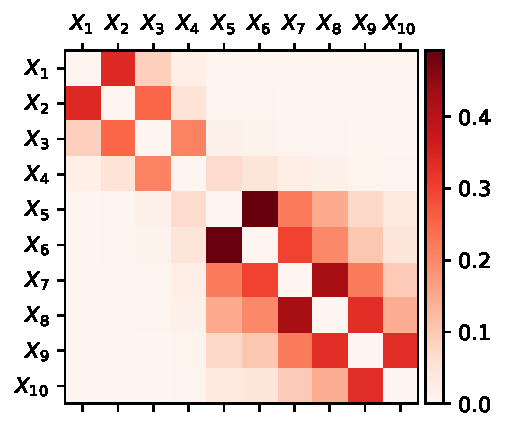
\includegraphics[width=.95\linewidth]{figures/Gaussian Chain Theoretical/G dir from symmetric G obs.pdf}
        \caption{$G_{dir}$}
        \label{subfig:Gaussian chain symmetric G_obs using correlation - G_dir}
    \end{subfigure}
    \\[\baselineskip]
    \begin{subfigure}[t]{0.49\textwidth}
        \centering
        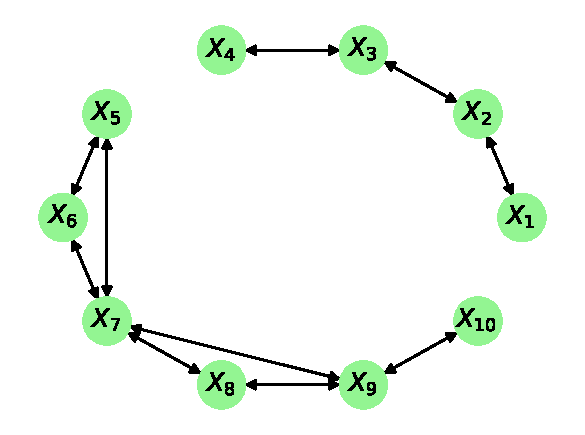
\includegraphics[width=.9\linewidth]{figures/Gaussian Chain Theoretical/Chain graph from symmetric G obs.pdf}
        \caption{$G_{dir}$ as a graph}
        % \label{}
    \end{subfigure}
    \caption{Using a symmetric $G_{obs}$ as shown in (a), we observe that higher order effects start to emerge as can be seen in (b). The main response is still in the superdiagonal and subdiagonal as we expect, where some similarity seems to bleed to nearby nodes/variables thus making the threshold used important for the resulting graph. For (c), a threshold $t=0.2$ was used to obtain a decent compromise between connectedness and denseness of the direct association.}
    \label{fig:Gaussian chain symmetric G_obs using correlation}
\end{figure}
% minimize error in g_dir from equation on error?
Finally, we try using the unscaled $G_{obs}$ in \autoref{eq:Gdir from Gobs}. Interestingly, we find that the true structure emerges as can be seen from \autoref{fig:Gaussian chain symmetric G_obs using correlation - unscaled}. Although the \textit{correlations} in \autoref{subfig:Gaussian chain symmetric G_obs using correlation - G_dir - unscaled} are not really correlations they do resemble those discovered in \autoref{subfig:Gaussian chain triangular G_obs using correlation - G_dir}. On closer inspection, it is not apparent how they are related except that it is a non-linear relationship. Although in this case it seemed to work not rescaling $G_{obs}$ in order to discover the causal structure we will in general not apply this to real world scenarios as the method is not well-defined in terms of assumptions and what the resulting $G_{dir}$ should be interpreted as.
\begin{figure}[ht]
    \centering
    \begin{subfigure}[t]{0.49\textwidth}
        \centering
        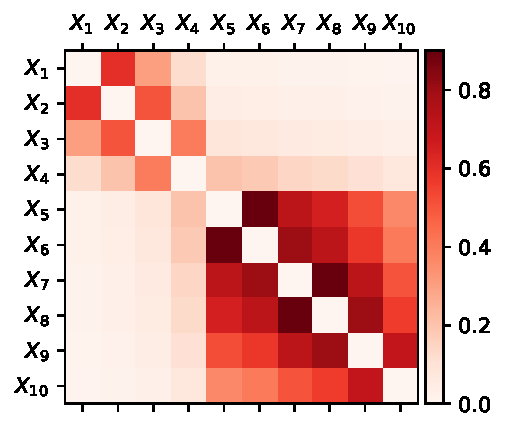
\includegraphics[width=.95\linewidth]{figures/Gaussian Chain Theoretical/symmetric G obs - unscaled.pdf}
        \caption{$G_{obs}$}
        % \label{}
    \end{subfigure}
    \hfill
    \begin{subfigure}[t]{0.49\textwidth}
        \centering
        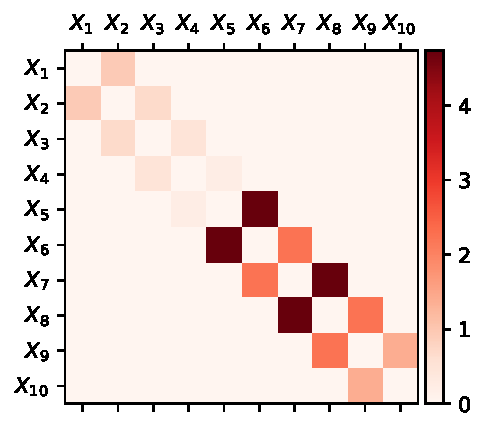
\includegraphics[width=.95\linewidth]{figures/Gaussian Chain Theoretical/G dir from symmetric G obs - unscaled.pdf}
        \caption{$G_{dir}$}
        \label{subfig:Gaussian chain symmetric G_obs using correlation - G_dir - unscaled}
    \end{subfigure}
    \\[\baselineskip]
    \begin{subfigure}[t]{0.49\textwidth}
        \centering
        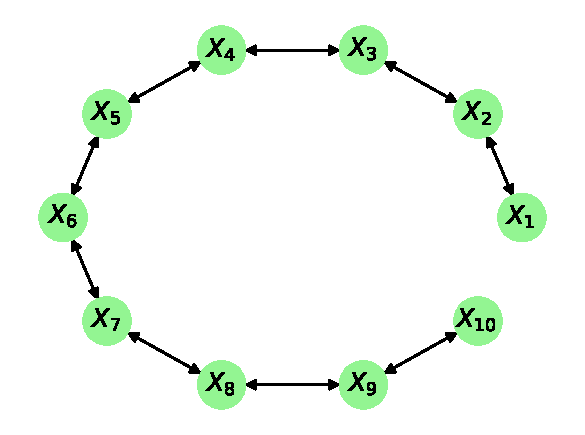
\includegraphics[width=.9\linewidth]{figures/Gaussian Chain Theoretical/Chain graph from symmetric G obs - unscaled.pdf}
        \caption{$G_{dir}$ as a graph}
        % \label{}
    \end{subfigure}
    \caption{Using an unscaled (symmetric) $G_{obs}$ results in a good recovery of the causal structure as seen in (b) and (c). However, at this point it is not clear whether it holds only for chains and using correlation or if it is a more general phenomenon.}
    \label{fig:Gaussian chain symmetric G_obs using correlation - unscaled}
\end{figure}
Thus, at this point we have a rather good understanding of how the method works on Gaussian chains if one uses correlation as a measure of association. Furthermore, if one knows (a plausible) topological ordering of the variables, we are able to perfectly rediscover the network of direct dependencies. However, as noted above, correlation is not always a good measure of similarity. Thus, we proceed experimenting with mutual information on the same Gaussian chain.

% Hvis den forkerte topologiske struktur benyttes, kan det give underlige resultater? -> Umiddelbart ja, for man ville ikke finde de rho i den originale definition, og der vil opstå effekter af et sådan forkert valgt topologisk orden.




\newpage

% Fejl regning for symmetrisk case? -> har undladt, da det er lidt mere komplekst og er nemmere at kvatificere med direkte udregninger
\subsection{Gaussian chain deconvolution using mutual information}
In this section, we continue the example from the previous section but instead of using correlation as a measure of similarity, we will use mutual information. Immediately, we note that mutual information or Copula entropy does not propagate as assumed in \autoref{eq:Gobs from Gdir}. As an example, from \autoref{prop:MI bivariate gaussian}, we know that the mutual information in the case of a Gaussian chain between a variable $X_i$ and the next variable $X_{i+1}$ is $-1/2 \log\left(1 - \rho_{i,i+1}^2\right)$ and similarly, using \autoref{eq:Gaussian chain G_obs triangular form}, we have that
$$I\left(X_i, X_{i+2}\right) = -\frac{1}{2} \log \left(1 - \rho_{i,i+1}^2 \rho_{i+1,i+2}^2\right)$$
Thus, if $G_{dir}$ is triangular, using \autoref{eq:Gobs from Gdir} we should observe the following at the $(i,i+2)$ entry of $G_{obs}$ instead
$$\frac{1}{4} \log\left(1 - \rho_{i,i+1}^2\right)\,\log\left(1 - \rho_{i+1,i+2}^2\right)$$
I.e. we make an error (which we could take to be the noise $N$ from \autoref{subseq:Robustness to noise}) for second order effects equal to
$$-\frac{1}{2} \log \left(1 - \rho_{i,i+1}^2 \rho_{i+1,i+2}^2\right) - \frac{1}{4} \log\left(1 - \rho_{i,i+1}^2\right)\,\log\left(1 - \rho_{i+1,i+2}^2\right)$$
In general, for a Gaussian chain, we have that
$$N_{i,j} = -\frac{1}{2} \log\left( 1 - \prod_{k=i+1}^{j} \rho_{k-1,k}^2\right) - \left(-\frac{1}{2}\right)^{j-i}\prod_{k=i+1}^{j} \log\left(1 - \rho_{k-1,k}^2\right)$$
As we will see in \autoref{fig:2 chain MI error} and \autoref{fig:3 and 4 chain MI error}, for Gaussian chains we can expect some of the same bleeding behavior as observed in \autoref{fig:Gaussian chain symmetric G_obs using correlation} where we did not use the topological ordering but based the deconvolution on correlation. In particular, from the figures below, we see that for $3$-chains, the error is in many cases close to $0$ and for most combinations of $\rho_{1,2}$ and $\rho_{2,3}$ less than $0.1$. Furthermore, we note that the errors are the largest when it is a strongly connected $3$-chain i.e. if both $\rho_{1,2}$ and $\rho_{2,3}$ are close to $1$ which again resemble the behavior seen in the case of a symmetrical $G_{obs}$ using correlation as the measure of association although in this case, the error does not propagate to the same extent which we shall also see shortly, when applying the deconvolution algorithm. Notice that as only the absolute value of the correlation matters, we only show the error for $\rho_{1,2}, \rho_{2,3} \geq 0$.
\begin{figure}[ht]
    \centering
    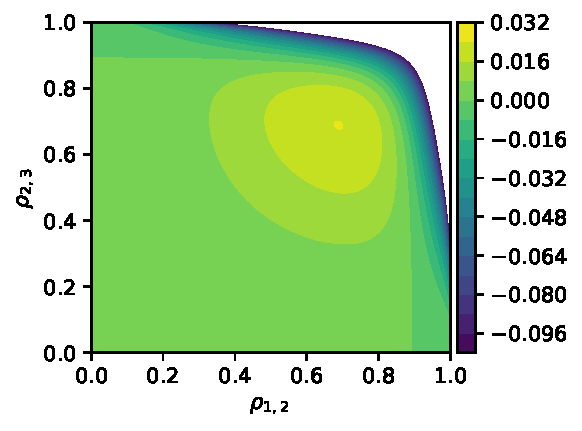
\includegraphics[width=.7\linewidth]{figures/Gaussian Chain Theoretical/2 chain error - MI.pdf}
    \caption{The error made by the assumption of $G_{obs}$ and $G_{dir}$ for second order observed effect. Although mutual information does not comply with the underlying assumptions, we observe that in the case of a Gaussian $2$-chain, we can expect the error to be relatively small.}
    \label{fig:2 chain MI error}
\end{figure}

We extend the above discussion to $4$- and $5$-chains (i.e. $j = i + 3$ and $j = i + 4$ in the above expression for $N_{ij}$) to see how the error propagates in more detail. This is shown in \autoref{fig:3 and 4 chain MI error} for three different scenarios of a $4$-chain and a single $5$-chain. In particular, as the error $N_{i,j}$ is symmetric in $\rho_{1,2}$, $\rho_{2,3}$ and $\rho_{3,4}$ (and $\rho_{4,5}$ in the case of a $5$-chain) and because it is hard to accurately show four or five dimensional surfaces, we keep to a fixed set of $\rho_{3,4}$ and $\rho_{4,5}$ when investigating. For the $4$-chain, choosing $\rho_{2,3} = 0.9$ (corresponding to mutual information about $0.8304$) approximately results in the same error as in \autoref{fig:2 chain MI error} and if $\rho_{2,3}$ is above e.g. $0.95$, we get a worse propagation of errors compared to the $3$-chain. Finally, from \autoref{subfig:Gaussian 5 chain MI error}, we see the same picture i.e. that keeping the correlations and hence information between subsequent variable low results in smaller errors in $G_{obs}$ and hence the inferred $G_{dir}$. Note that under the assumption of a topological ordering such that $G_{obs}$ is strictly upper triangular results in $\rho\left(G_{obs}\right) = 0$ such that no rescaling is necessary (although different choices of the base of the logarithm would have an effect on how much higher order associations influence $G_{dir}$).

% Ud fra plots, kan vi konkludere at fejlene ved at bruge den transformere G_obs ud fra correlation ikke er så lang væk fra det man ville få ud fra convolution af G_dir (under antagelse af at summen convergerer -> det gør den altid, fordi G_dir er strengt øvre trekant, så "inf" sum er faktisk begrænset/endelig)

Having obtained a good understanding of how shifting to mutual information instead of correlation in the case of Gaussian chains, we continue with the above example now using mutual information as the elements of $G_{obs}$ based on the correlation matrix from the previous section. Using a triangular $G_{obs}$ we observe similar behavior to that of original example using a triangular $G_{obs}$ but with correlation as can be seen from \autoref{fig:Gaussian chain triangular G_obs using mutual information}. In particular, we do not observe the same magnitude of bleeding effects as in \autoref{fig:Gaussian chain symmetric G_obs using correlation}. However, we observe
\begin{figure}[H]
    \centering
    \begin{subfigure}[t]{0.49\textwidth}
        \centering
        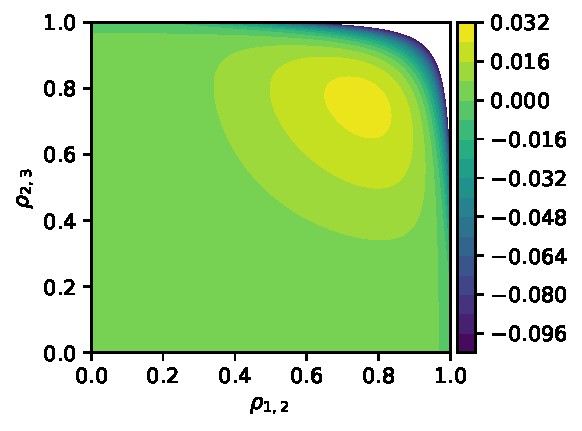
\includegraphics[width=.95\linewidth]{figures/Gaussian Chain Theoretical/3 chain error - MI - rho3 0_7.pdf}
        \caption{$4$-chain $\rho_{3,4} = 0.7$}
    \end{subfigure}
    \hfill
    \begin{subfigure}[t]{0.49\textwidth}
        \centering
        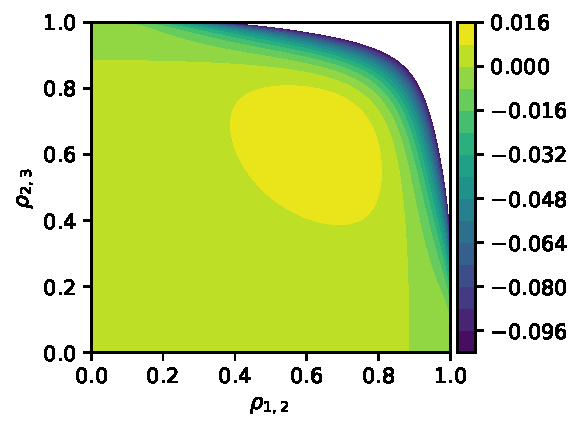
\includegraphics[width=.95\linewidth]{figures/Gaussian Chain Theoretical/3 chain error - MI - rho3 0_9.pdf}
        \caption{$4$-chain $\rho_{3,4} = 0.9$}
    \end{subfigure}
    \\[\baselineskip]
    \begin{subfigure}[t]{0.49\textwidth}
        \centering
        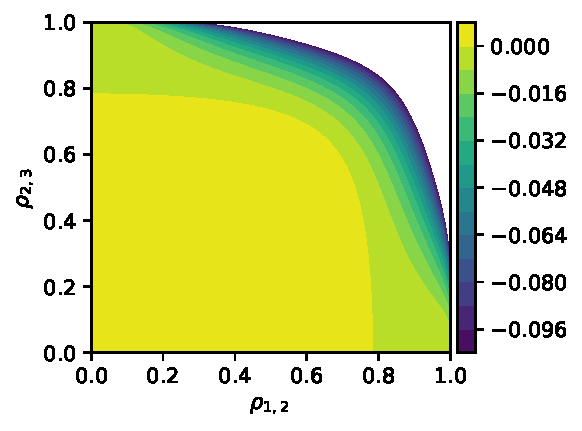
\includegraphics[width=.95\linewidth]{figures/Gaussian Chain Theoretical/3 chain error - MI - rho3 0_95.pdf}
        \caption{$4$-chain $\rho_{3,4} = 0.95$}
    \end{subfigure}
    \hfill
    \begin{subfigure}[t]{0.49\textwidth}
        \centering
        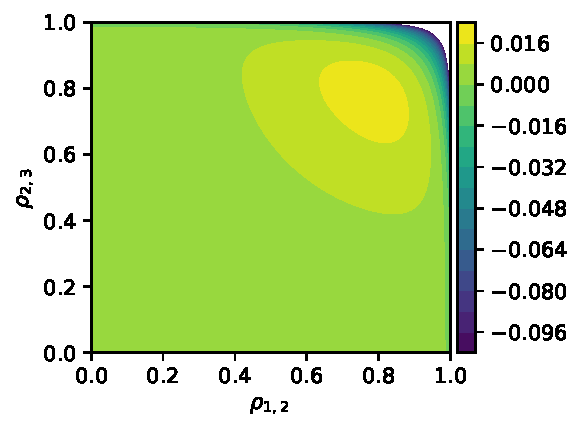
\includegraphics[width=.95\linewidth]{figures/Gaussian Chain Theoretical/4 chain error - MI - rho3 0_85 rho4 0_6.pdf}
        \caption{$5$-chain $\rho_{3,4} = 0.85$, $\rho_{4,5} = 0.6$}
        \label{subfig:Gaussian 5 chain MI error}
    \end{subfigure}
    \caption{Errors of convolving mutual information along a $4$-chain (a), (b), (c) and a $5$-chain (d). Due to symmetry in the expression of the error, only the first $2$ links i.e. $\rho_{1,2}$ and $\rho_{2,3}$ are varied on $[0,1]$ respectively. Only positive correlations are shown as the sign of the correlation cancels in the expression for the error. We note that large correlations and hence large mutual information on each edge results in larger error. In particular, when not too many of the links are strong, we have almost $0$ error.}
    \label{fig:3 and 4 chain MI error}
\end{figure}
the same tendency to miss weak connections as was also observed in \autoref{fig:Gaussian chain symmetric G_obs using correlation}. All in all, we get very good results using a triangular $G_{obs}$ even though mutual information does not have the same properties as correlation. In particular, this is what we expected as we have only used $\rho_{i,i+1} \leq 0.9$, from the above investigation of the error.
\begin{figure}[H]
    \centering
    \begin{subfigure}[t]{0.49\textwidth}
        \centering
        \includegraphics[width=.95\linewidth]{figures/Gaussian Chain Theoretical/triangular G obs - MI.pdf}
        \caption{$G_{obs}$}
    \end{subfigure}
    \hfill
    \begin{subfigure}[t]{0.49\textwidth}
        \centering
        \includegraphics[width=.95\linewidth]{figures/Gaussian Chain Theoretical/G dir from triangular G obs - MI.pdf}
        \caption{$G_{dir}$}
    \end{subfigure}
    \\[\baselineskip]
    \begin{subfigure}[t]{0.49\textwidth}
        \centering
        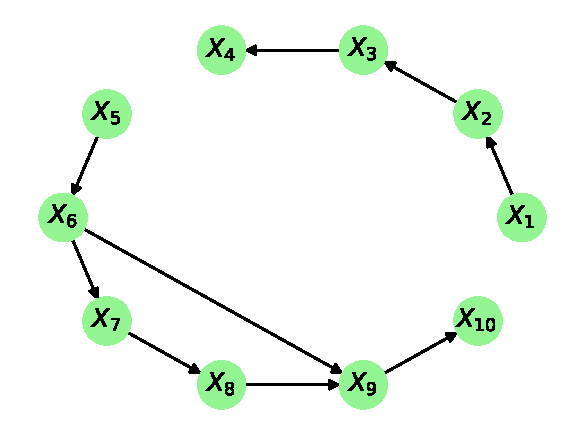
\includegraphics[width=.9\linewidth]{figures/Gaussian Chain Theoretical/Chain graph from triangular G obs - MI - cutoff 2_1e-2.pdf}
        \caption{$G_{dir}$ from $t = 2.1\cdot 10^{-2}$}
    \end{subfigure}
    \hfill
    \begin{subfigure}[t]{0.49\textwidth}
        \centering
        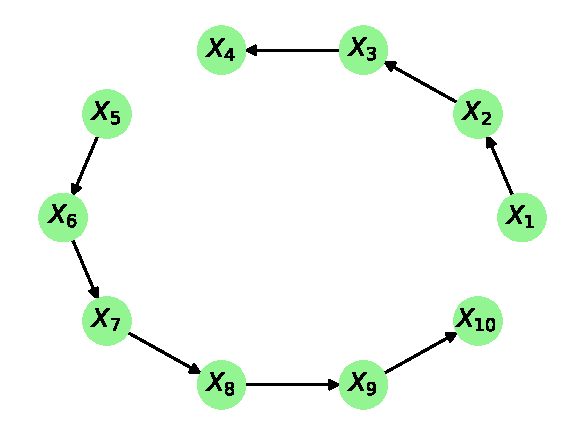
\includegraphics[width=.9\linewidth]{figures/Gaussian Chain Theoretical/Chain graph from triangular G obs - MI - cutoff 4_6e-2.pdf}
        \caption{$G_{dir}$ from $t = 4.6\cdot 10^{-2}$}
    \end{subfigure}
    \caption{Using mutual information as the measure of similarity as well as assuming a topological order i.e. making $G_{obs}$ strictly triangular as seen in (a) we almost perfectly infer $G_{dir}$ as seen in (b) except for $\left[G_{dir}\right]_{6,9}$. Choosing cutoffs $t = 2.1\cdot 10^{-2}$ (c) and $t = 4.6\cdot 10^{-2}$ (d) it is clear that adjusting the threshold we can get a better result than using a symmetric $G_{obs}$ with correlation.}
    \label{fig:Gaussian chain triangular G_obs using mutual information}
\end{figure}
Finally, we use the corresponding symmetric $G_{obs}$ (rescaled such that the largest absolute eigenvalue of $G_{dir}$ is $0.99$) which results in $G_{dir}$ and the graph using a threshold $t=4.88\cdot 10^{-2}$ shown in \autoref{fig:Gaussian chain symmetric G_obs using mutual information}. Again, we observe some bleeding on the more strongly connected sub-chain as with the symmetric $G_{obs}$ using correlation in \autoref{fig:Gaussian chain symmetric G_obs using correlation}. Again, we observe comparable results and note that increasing the threshold would disconnect $X_3$ and $X_4$ before removing the higher order effects.
\begin{figure}[ht]
    \centering
    \begin{subfigure}[t]{0.49\textwidth}
        \centering
        \includegraphics[width=.95\linewidth]{figures/Gaussian Chain Theoretical/symmetric G obs - MI.pdf}
        \caption{$G_{obs}$}
    \end{subfigure}
    \hfill
    \begin{subfigure}[t]{0.49\textwidth}
        \centering
        \includegraphics[width=.95\linewidth]{figures/Gaussian Chain Theoretical/G dir from symmetric G obs - MI.pdf}
        \caption{$G_{dir}$}
    \end{subfigure}
    \\[\baselineskip]
    \begin{subfigure}[t]{0.49\textwidth}
        \centering
        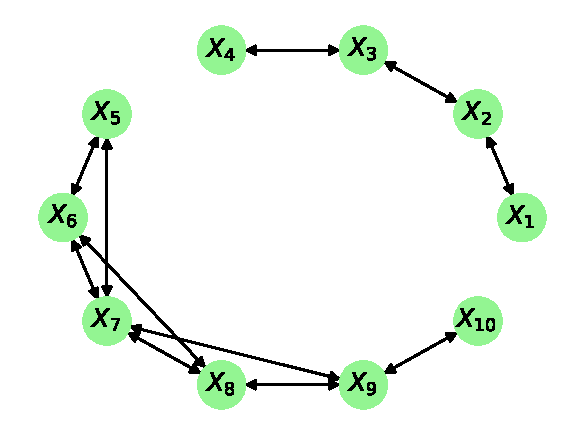
\includegraphics[width=.9\linewidth]{figures/Gaussian Chain Theoretical/Chain graph from symmetric G obs - MI - cutoff 4_88e-2.pdf}
        \caption{$G_{dir}$ as a graph}
    \end{subfigure}
    \caption{Using a symmetric $G_{obs}$ containing the observed mutual information (a) we infer a $G_{dir}$ (b) comparable to that if we had used correlation instead. Choosing the threshold $t = 4.88 \cdot 10^{-2}$ seem a good compromise between connectedness and density resulting in an almost identical discovered network structure to that of using a symmetric correlation $G_{obs}$.}
    \label{fig:Gaussian chain symmetric G_obs using mutual information}
\end{figure}

In conclusion, we have seen what errors can arise in the discovered network using both correlation and mutual information as the measure of association. Namely, long strongly connected chains seem to be a problem if one does not know a topological ordering of the variables, in which case these are heavily reduced  as seen in \autoref{fig:Gaussian chain triangular G_obs using correlation} and \autoref{fig:Gaussian chain triangular G_obs using mutual information}. Thus, we proceed in the next section by considering a more complicated underlying (Gaussian) network to observe if other unwanted effects can occur and if a topological ordering is necessary if the network is not simply a path.




\newpage
\section{Directed acyclic Gaussian graphs}\label{sec:General Gaussian graph}
In this section, we will expand on the results from the previous section by considering a more general structure. In particular, let $\mathcal{G}$ be a directed acyclic graph with nodes corresponding to variables from a random vector $\boldsymbol X$ with directed edges indicating direct dependencies. Clearly, such a DAG has a topological ordering and as such we shall index the variables $1$ through $d$ such that if the index of a variable is $i$, and $j$ is the index of another element of the random vector $\boldsymbol X$, then $i < j$ implies there is no (directed) path from $j$ to $i$. Note that since a topological ordering is not necessarily unique, we can not infer that there is a (directed) path from $i$ to $j$ or even if $k$ is reachable form $j$ (i.e. there exists a path from $j$ to $k$) it does not follow that $k$ is reachable from $i$. In \autoref{fig:General gaussian graph illustration} a subset of such a DAG is shown with a possible labelling where $i < j$ and $k_m < k_n$ when $m < n$. It is then the weights along these directed edges which we will once again call $G_{dir}$ that we wish to infer based on the transitive closure. As an example, from \autoref{fig:General gaussian graph illustration}, the transitive closure would result in an observed similarity between $i$ and $j$ although no $1$ path i.e. single direct edge connects the two variables.
\begin{figure}[ht]
    \centering
    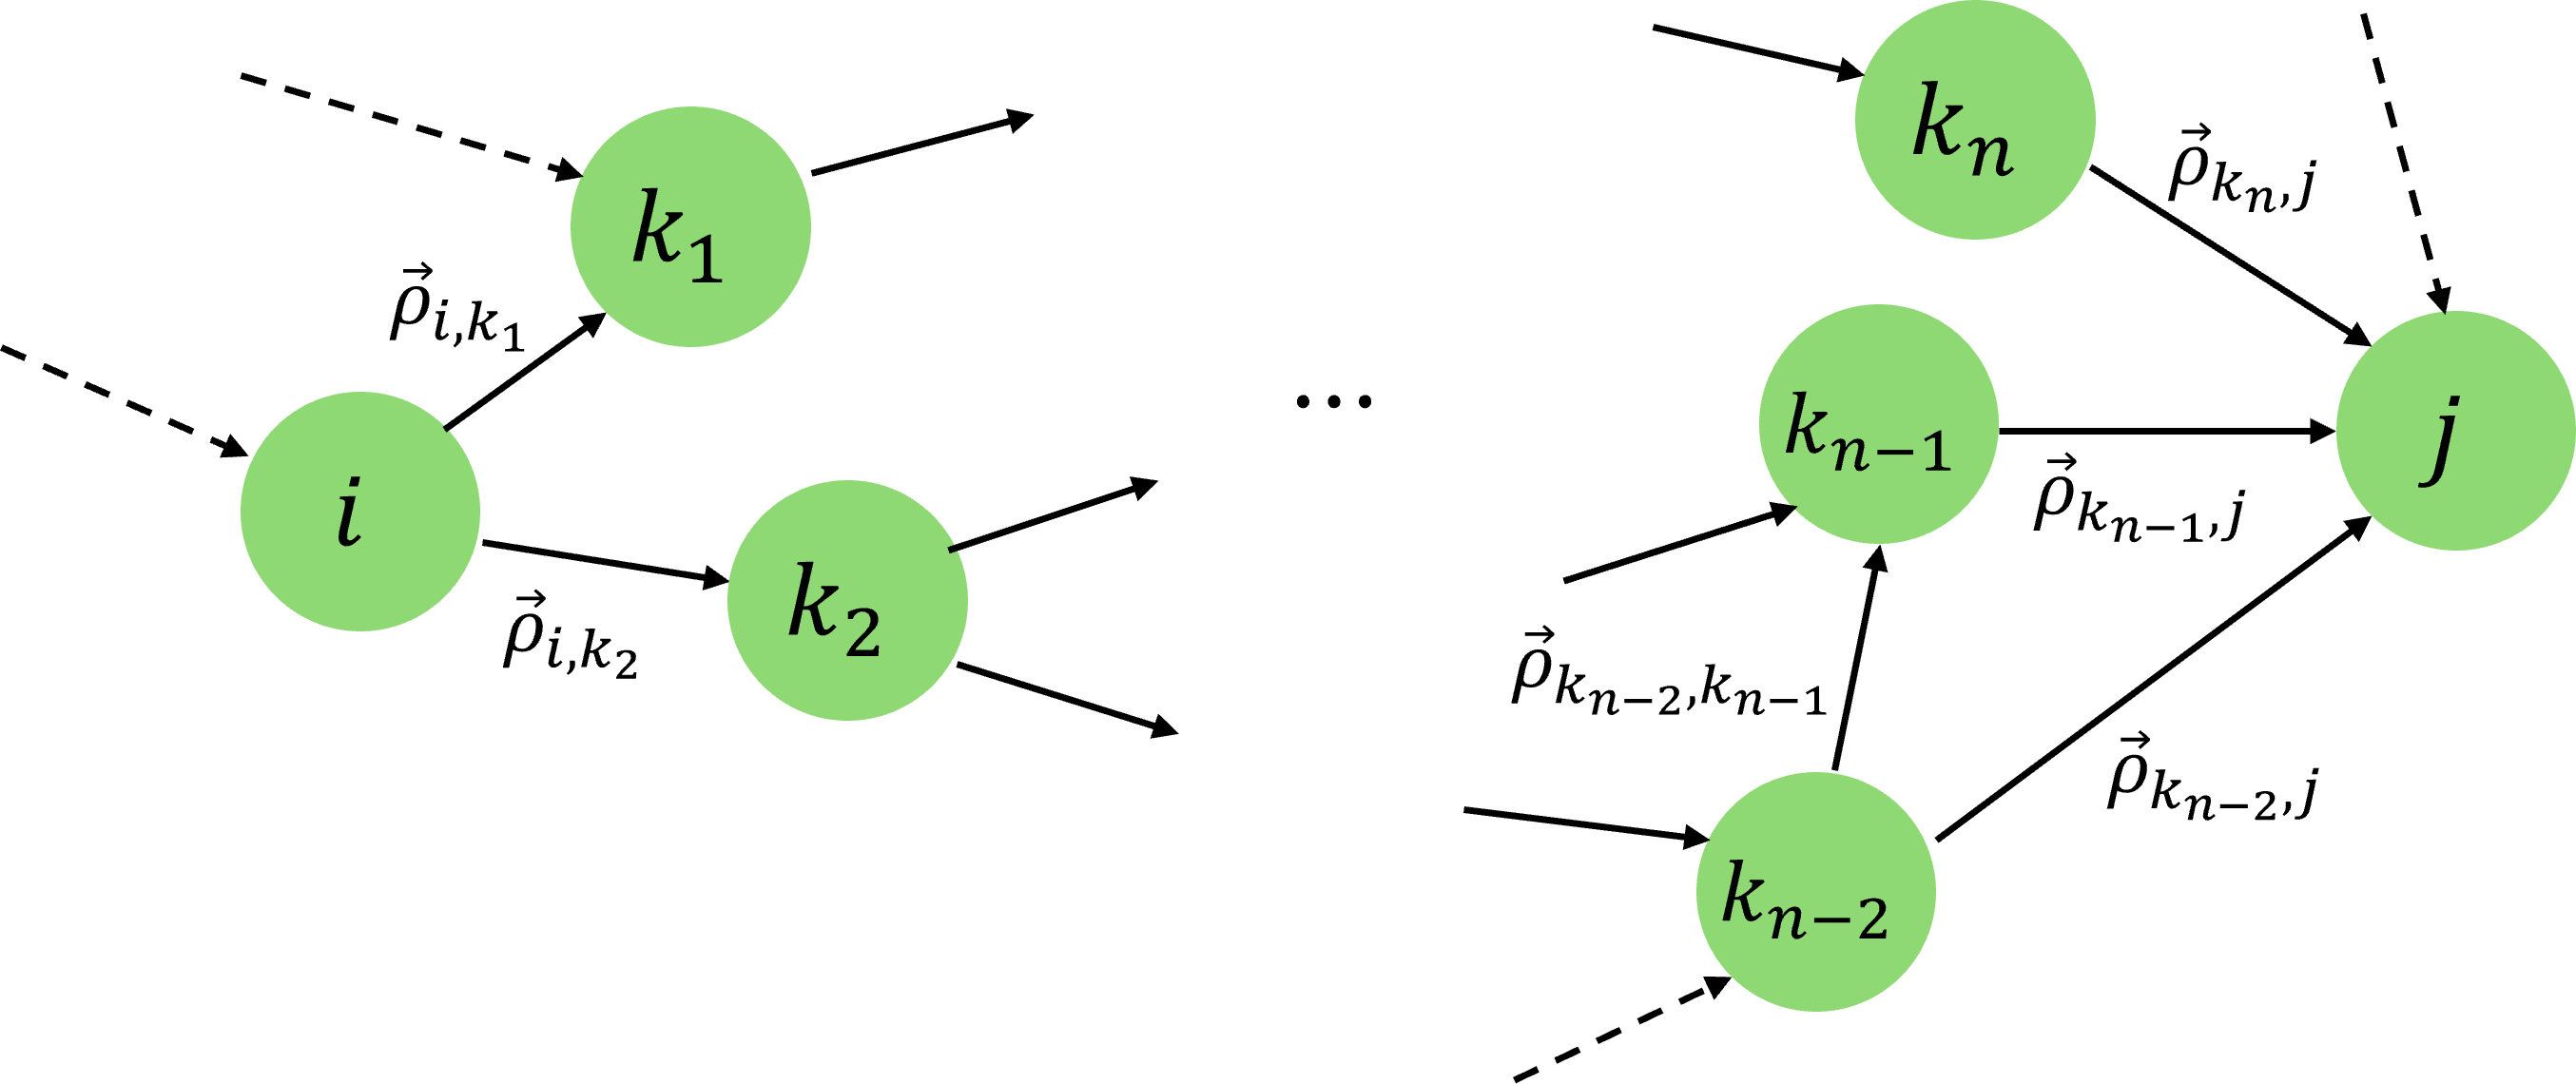
\includegraphics[width = .7\linewidth]{figures/ND examples/Gaussian graph illustration.png}
    \caption{A general (linear) network represented as a DAG. The directed edge weights $\vec{\rho}_{k,l}$ specify how much the variable index $k$ make up of variable $l$. Although $i$ and $j$ are not directly connected, multiple paths may exist between the two nodes, making the propagation of similarity more complex from that of a chain.}
    \label{fig:General gaussian graph illustration}
\end{figure}
From the definition of the labels, it is clear that $G_{dir}$ is once again strictly upper triangular as entries below the diagonal corresponds to edges going from a random variable with an index $i$ to another random variable with index $j$ such that $i > j$ which is clearly a contradiction. Also, the diagonal elements are $0$ as there can not be any loops in DAGs.

Similarly to the definition of (Gaussian) chains, based on $d$ independent (or even just pairwise uncorrelated) random variables $Z_i$ we can define a general network of random variables $X_i$ based on $\boldsymbol Z$ in the following way
\begin{equation}\label{eq:Gaussian network in terms of Z}
    \begin{split}
        X_1 & = Z_1                                                      \\
        X_2 & = \vec{\rho}_{1,2} X_1 + \sqrt{1 - \vec{\rho}_{1,2}^2} Z_2 \\
        X_3 & = \vec{\rho}_{1,3} X_1 + \vec{\rho}_{2,3} X_2 + c_3 Z_3    \\
            & \vdots                                                     \\
        X_d & = \sum_{k < d} \vec{\rho}_{k,d} X_k + c_d Z_d
    \end{split}
\end{equation}
where $c_i$ is chosen such that $\text{Var}\left(X_i\right) = 1$. This is done to make the analysis later on simpler as then covariance and correlation are equal and $\vec{\rho}_{i,j}$ becomes the \textit{direct} correlation between the variables indexed $i$ and $j$ as shown in \autoref{fig:General gaussian graph illustration}. Of course, for the variance of each random variable to be $1$ there must be some constraints on the chosen $\vec{\rho}_{i,j}$ such as neither one of them can exceed $1$ in absolute value. Furthermore, consider the following bound on the variance of $X_i$ assuming $c_k$ for $k < i$ have been chosen such that $\text{Var}\left(X_k\right) = 1$.
\begin{equation}\label{eq:bound on variance for network variable from the sum of ingoing weights}
    \begin{aligned}
        \text{Var}\left[X_i\right] & = \sum_{k < i} \vec{\rho}_{k,i}^2 + 2\sum_{k < l < i} \vec{\rho}_{k,i} \vec{\rho}_{l,i} \text{Cov} \left[X_k,X_l\right] + c_i^2 \\
                                   & \leq  \sum_{k < i} \vec{\rho}_{k,i}^2 + 2\sum_{k < l < i} \vec{\rho}_{k,i} \vec{\rho}_{l,i} + c_i^2                             \\
                                   & = \left(\sum_{k < i} \rho_{k,i}\right)^2 + c_i^2
    \end{aligned}
\end{equation}
where we have used that $Z_i$ is uncorrelated with $X_k$ for $k < i$ and that the covariance between variables with variance $1$ is at most $1$ to obtain the inequality. Hence, choosing the sum of the ingoing edges to be at most $1$ for every node ensures that the constants $c_i$ for $i\in\left\{2,\dots, d\right\}$ exist in order to make the variance of each $X_i$ $1$. This, we will use in the following example to easily build a network such that $\vec{\rho}_{i,j}$ is the pure correlation.

However, before constructing an example and using bot correlation and mutual information we must determine the theoretical $G_{obs}$ for both cases. To do this, we shall consider the $(i,j)$ element of $G_{obs}$ when using correlation as a measure of similarity and later use mutual information based on these correlations and \autoref{prop:MI bivariate gaussian} in the case of $\boldsymbol Z$ being a Gaussian random vector. To calculate $\left[G_{obs}\right]_{i,j}$ we shall consider the immediate predecessors to node $j$ in the graph $\mathcal{G}$ corresponding to \autoref{eq:Gaussian network in terms of Z}. The immediate predecessors or \textit{in-neighbors} of a node $j$ is denoted $N^-\left(X_j\right)$ or in shorthand notation $N^-_j$. An example of this is shown in \autoref{fig:Gaussian graph illustration - immediate predecessor} where the in-neighbors of $j$ has been marked in red. With this notation, we proceed with the computation of the $(i,j)$ entry of $G_{obs}$ which is the covariance between $X_i$ and $X_j$ when $i < j$ and $0$ elsewhere.
\begin{figure}[ht]
    \centering
    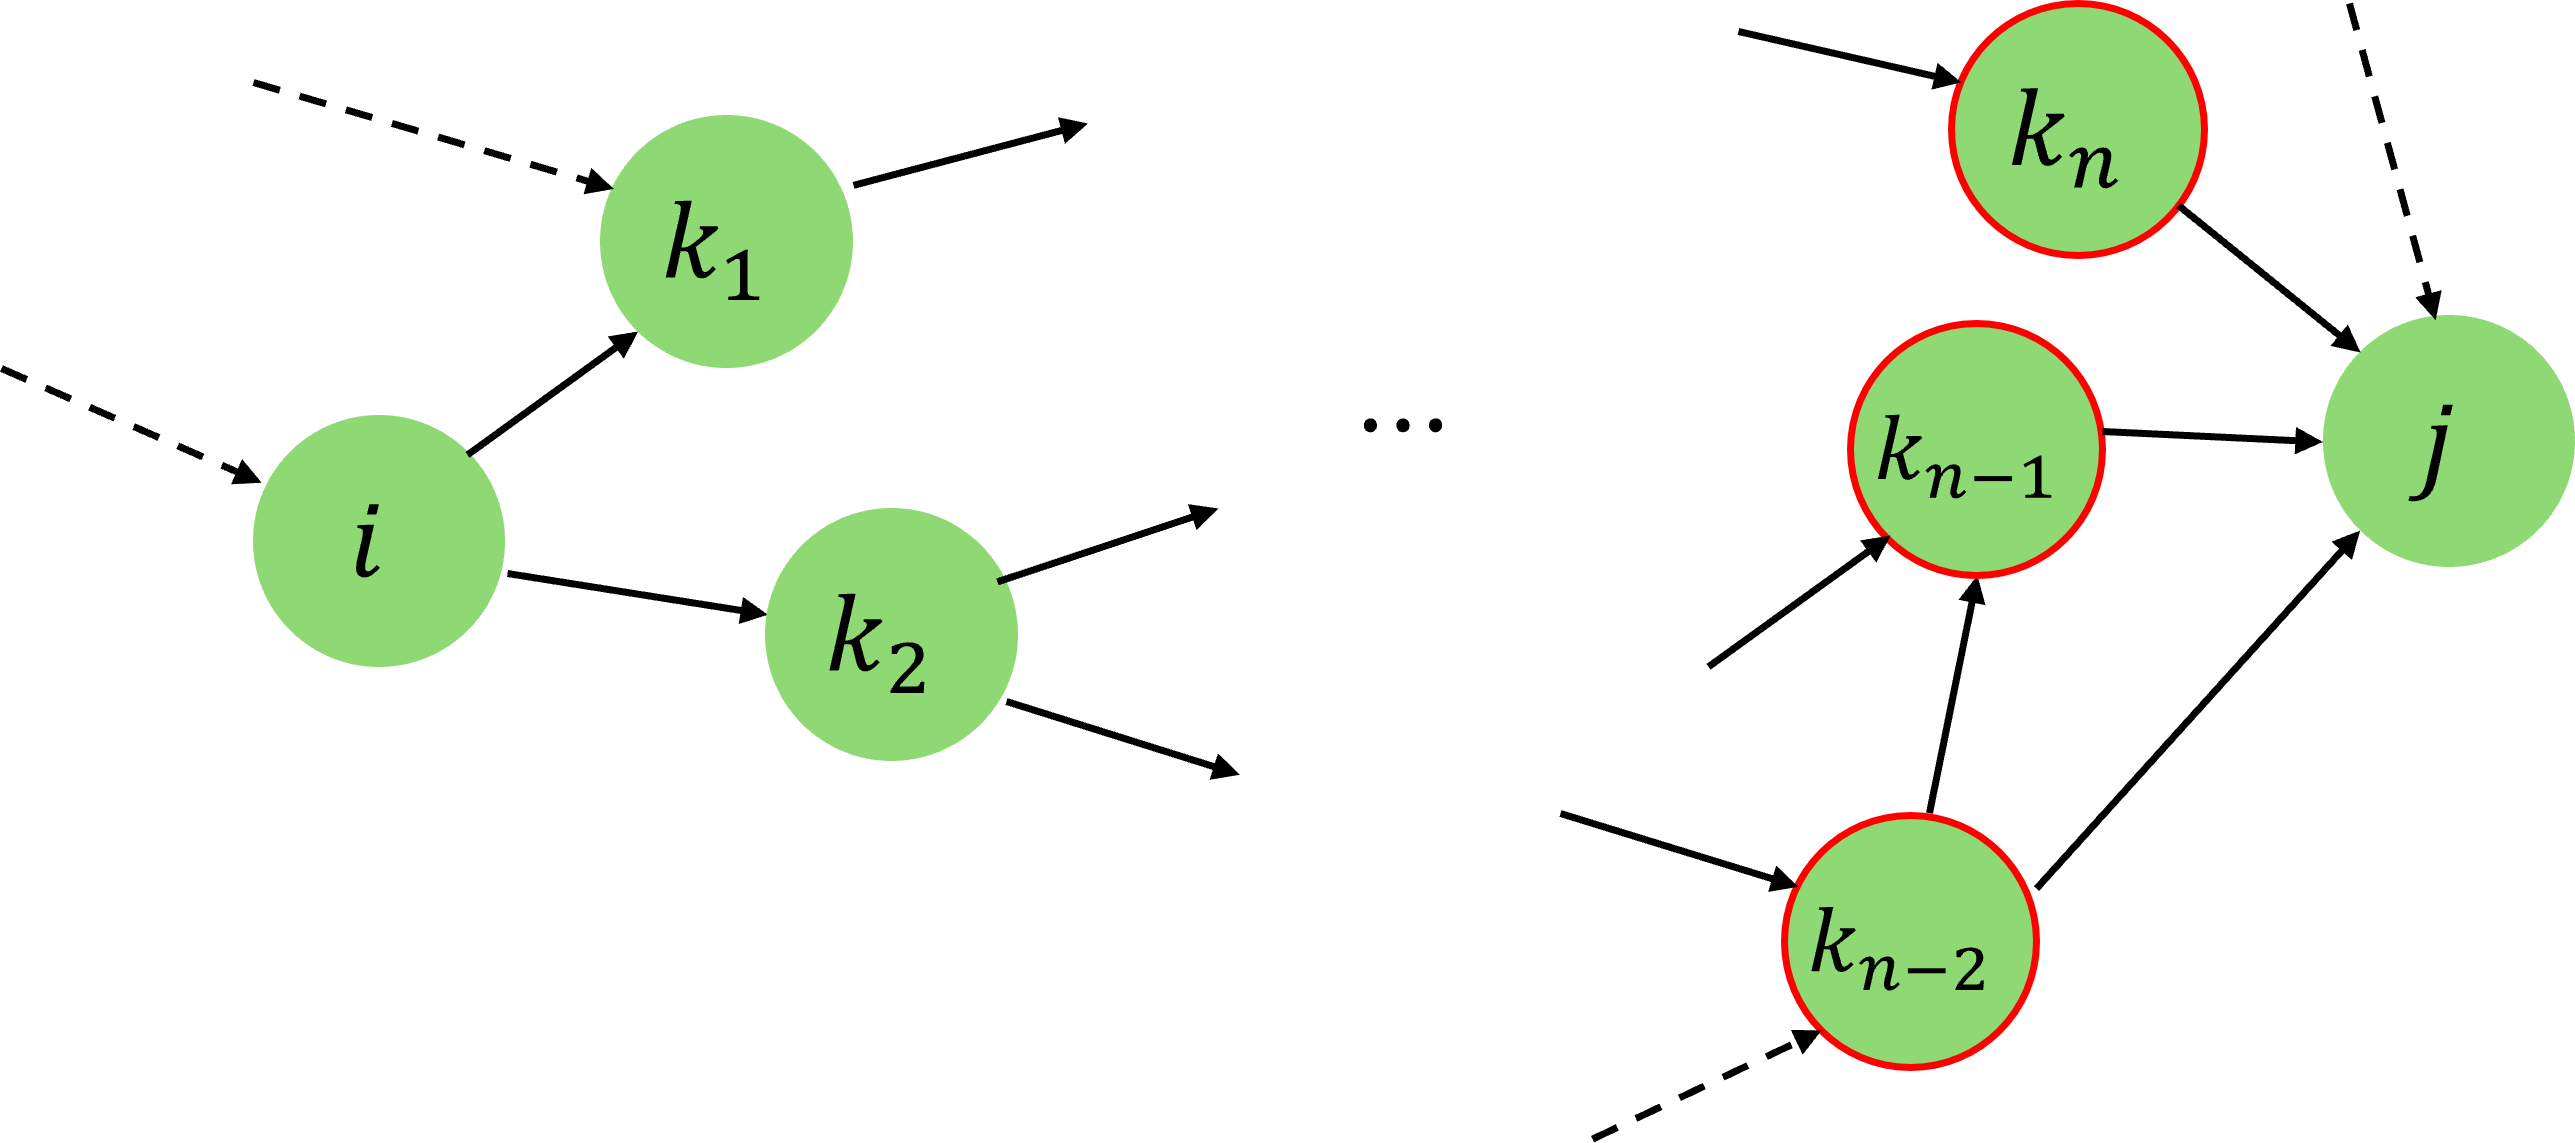
\includegraphics[width = .7\linewidth]{figures/ND examples/Gaussian graph illustration - immediate predecessor.png}
    \caption{For node $j$, the set $N^-_j$ is illustrated with red borders. It is exactly the set of nodes going directly into $j$. We note that an in-neighbor $l$ of in-neighbor $k$ of node $j$ can also be an in-neighbor of $j$ i.e. $l$ can influence both $k$ and $j$ whilst $k$ also directly influenced $j$. It is in particular these direct dependencies we want to be sure of as their existence makes the network more complex but failing to discover these can lead to a significant reduction in prediction accuracy.}
    \label{fig:Gaussian graph illustration - immediate predecessor}
\end{figure}
\begin{equation}
    \begin{split}
        \left[G_{obs}\right]_{i,j} & = \text{Cov}\left[X_i , \sum_{k \in N^-_j} \vec{\rho}_{k,j} \, X_k + c_j Z_j\right] \\
                                   & = \text{Cov}\left[X_i , \sum_{k \in N^-_j} \vec{\rho}_{k,j} \, X_k\right]           \\
                                   & = \sum_{k \in N^-_j}\vec{\rho}_{k,j} \text{Cov}\left[X_i, X_k\right]                \\
                                   & = \sum_{k \in 1}^{j-1} \vec{\rho}_{k,j} \text{Cov}\left[X_i, X_k\right]             \\
                                   & = \vec{\rho}_{i,j} + \sum_{k \in 1}^{d} \vec{\rho}_{k,j} \left[G_{obs}\right]_{i,k}
    \end{split}
\end{equation}
For the fourth equality, we have used that $\vec{\rho}_{k,j} = 0$ whenever $k \not\in N^-_j$ which again for the fifth equality holds for any $k \geq j$. Furthermore, since $\left[G_{obs}\right]_{i,i} = 0$ we need to add $\vec{\rho}_{i,j}$ to make the final equality hold. It is clear that the above can also be expressed as a matrix equation, namely
$$G_{obs} = G_{obs}G_{dir} + G_{dir}$$
Hence, as $G_{dir}$ is strictly upper triangular thus making $I - G_{dir}$ invertible, we can directly express $G_{obs}$ in terms of $G_{dir}$. We find that
$$G_{obs} = G_{dir} \left(I - G_{dir}\right)^{-1}$$
which we recognize as \autoref{eq:Gobs from Gdir} hence also for a general network (and not just a chain), using correlation and knowing/assuming a topological order of the random variables we are able to perfectly rediscover $G_{dir}$ from $G_{obs}$.

With the above, we then define an example Gaussian network with the following weights and shown in \autoref{fig:Gaussian network example - ground truth} to get a better understanding of this example hopefully should reappear after deconvolution using both correlation and mutual information respectively.
\begin{equation}\label{eq:example Gaussian network}
    \begin{aligned}
        \vec{\rho}_{1,2} & = 0.7, & \vec{\rho}_{5,6}  & = 0.5, & \vec{\rho}_{2,7}  & = 0.3 \\
        \vec{\rho}_{6,7} & = 0.3, & \vec{\rho}_{6,8}  & = 0.7, & \vec{\rho}_{4,9}  & = 0.3 \\
        \vec{\rho}_{8,9} & = 0.3, & \vec{\rho}_{7,10} & = 0.4, & \vec{\rho}_{9,10} & = 0.2
    \end{aligned}
\end{equation}
In particular, from \autoref{eq:bound on variance for network variable from the sum of ingoing weights} and \autoref{fig:2 chain MI error} and \autoref{fig:3 and 4 chain MI error}, we suspect that the bleeding effects observed for the Gaussian chain won't appear to the same extent in this case.
\begin{figure}[ht]
    \centering
    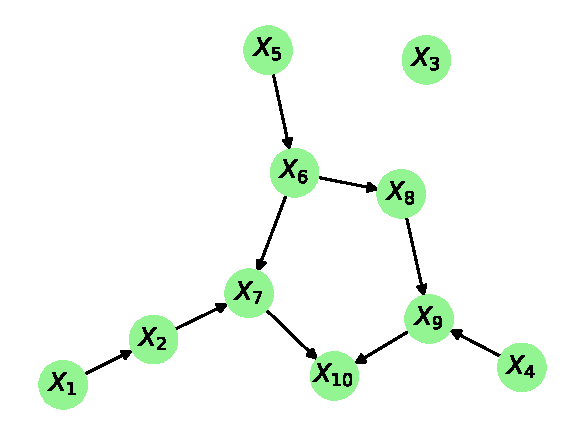
\includegraphics[width = .6\linewidth]{figures/Gaussian Network Theoretical/Network graph - ground truth.pdf}
    \caption{The graph defined in \autoref{eq:example Gaussian network}. Note that $X_3$ is neither influenced nor influences any other variable. It is of course in our interest to accurately tell if $X_3$ should be considered if we try to infer a probability distribution on e.g. $X_{10}$ given observations of the other variables.}
    \label{fig:Gaussian network example - ground truth}
\end{figure}

Applying the deconvolution algorithm, we obtain the results in \autoref{fig:Gaussian network triangular G_obs using correlation} which trivially, from the above analysis on $G_{obs}$, results in a perfect reconstruction of the network. If instead, we do not assume a topological structure, we can also recover the structure, although we need to tune the threshold as can be seen from \autoref{fig:Gaussian network symmetric G_obs using correlation}. Tuning the $\alpha$ and $\beta$ did not have much of an effect. Actually, decreasing $\beta$ seemed to worsen the results which is also in line with our expectations as choosing smaller $\beta$ skews the effects of higher order interactions. Thus, it is primarily the threshold that we want to tune in this case and choosing $t = 1.18 \cdot 10^{-1}$ we accurately infer the network structure contrary to the results from the Gaussian chain. However, we still observe second order effects i.e. the edge between $X_5$ and $X_8$ which was also the case in \autoref{fig:Gaussian chain symmetric G_obs using correlation}
\begin{figure}[ht]
    \centering
    \begin{subfigure}[t]{0.49\textwidth}
        \centering
        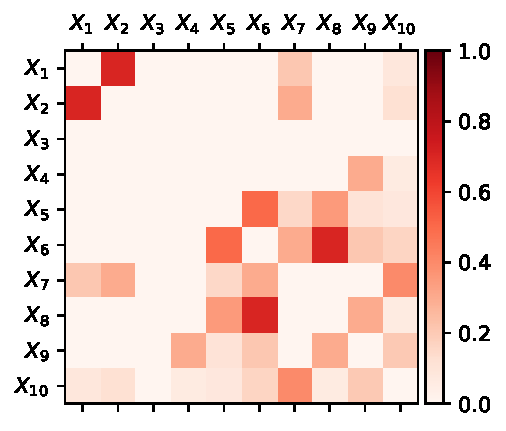
\includegraphics[width=.95\linewidth]{figures/Gaussian Network Theoretical/symmetric G obs - cor.pdf}
        \caption{$G_{obs}$}
    \end{subfigure}
    \hfill
    \begin{subfigure}[t]{0.49\textwidth}
        \centering
        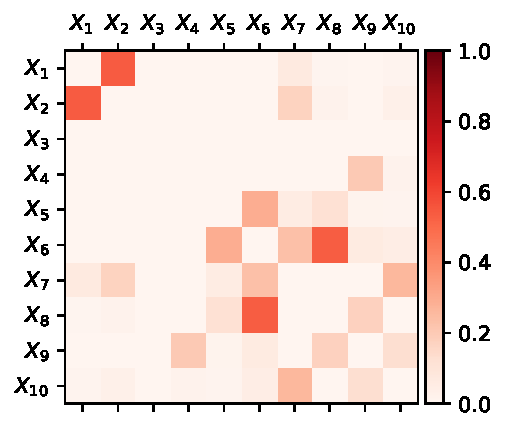
\includegraphics[width=.95\linewidth]{figures/Gaussian Network Theoretical/G dir from symmetric G obs - cor.pdf}
        \caption{$G_{dir}$}
    \end{subfigure}
    \\[\baselineskip]
    \begin{subfigure}[t]{0.49\textwidth}
        \centering
        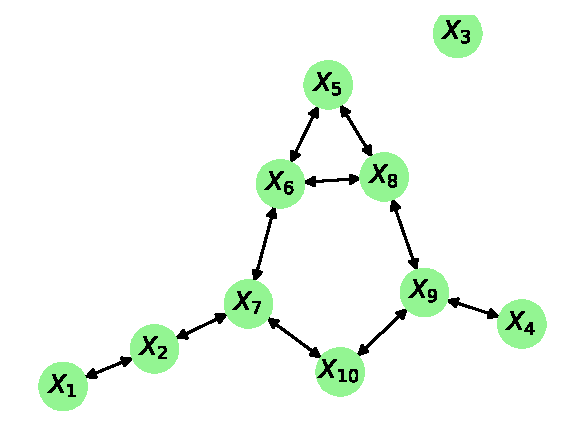
\includegraphics[width=.9\linewidth]{figures/Gaussian Network Theoretical/Graph from symmetric G obs - cor - cutoff 6_4e-2.pdf}
        \caption{$G_{dir}$  from $t = 6.4 \cdot 10^{-2}$}
    \end{subfigure}
    \hfill
    \begin{subfigure}[t]{0.49\textwidth}
        \centering
        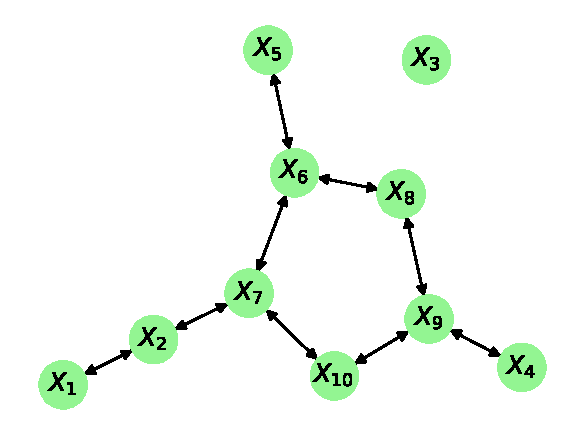
\includegraphics[width=.9\linewidth]{figures/Gaussian Network Theoretical/Graph from symmetric G obs - cor - cutoff 1_18e-1.pdf}
        \caption{$G_{dir}$ from $t = 1.18 \cdot 10^{-1}$}
    \end{subfigure}
    \caption{Not knowing the topological structure and thus using a symmetric $G_{obs}$ (a) we obtain the $G_{dir}$ in (b). Clearly, there is some bleeding, but choosing the threshold $t = 1.18 \cdot 10^{-1}$ we can accurately rediscover the network structure up to a direction on the edges. As with the previous example of Gaussian chains, we observe some tendency to inaccurately filter out second order effects as can be seen in (c) where $X_5$ and $X_8$ is connected.}
    \label{fig:Gaussian network symmetric G_obs using correlation}
\end{figure}
Finally, before continuing with results regarding the different methods for estimating mutual information, we present the results from above using mutual information instead of correlation as the measure of similarity. Namely, once again assuming the topological order such that $G_{obs}$ is strictly upper triangular and hence no need for rescaling we get the results shown in \autoref{fig:Gaussian network tringular G_obs using mutual information}. As expected, we observe on par performance to using correlation. Only the edge from $5$ to $8$ being almost as strong as $9$ to $10$ could be a problem i.e. choosing a threshold a little larger than $t = 1.7 \cdot 10^{-2}$ (which is quite small and has been used for \autoref{subfig:Gaussian network tringular G_obs using mutual information - t 1_7e-2}) would have resulted in an edge from $X_5$ to $X_8$. Hence, in a real world example we might have chosen to either leave out both edges which depending on the scenario may or may not be an acceptable error or include the both of them.
\begin{figure}[ht]
    \centering
    \begin{subfigure}[t]{0.49\textwidth}
        \centering
        \includegraphics[width=.95\linewidth]{figures/Gaussian Network Theoretical/triangular G obs - MI.pdf}
        \caption{$G_{obs}$}
    \end{subfigure}
    \hfill
    \begin{subfigure}[t]{0.49\textwidth}
        \centering
        \includegraphics[width=.95\linewidth]{figures/Gaussian Network Theoretical/G dir from triangular G obs - MI.pdf}
        \caption{$G_{dir}$}
    \end{subfigure}
    \\[\baselineskip]
    \begin{subfigure}[t]{0.49\textwidth}
        \centering
        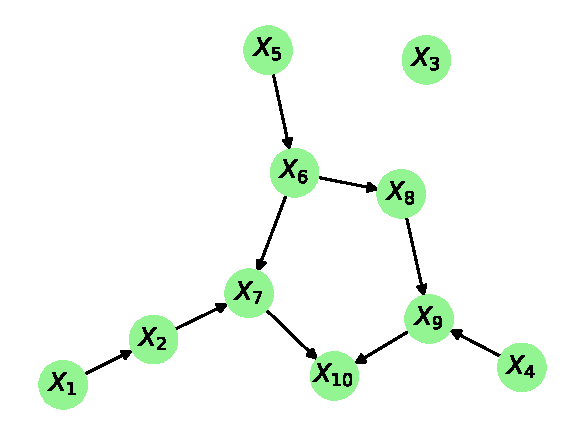
\includegraphics[width=.9\linewidth]{figures/Gaussian Network Theoretical/Graph from triangular G obs - MI - cutoff 1_7e-2.pdf}
        \caption{$G_{dir}$ as a graph}
        \label{subfig:Gaussian network tringular G_obs using mutual information - t 1_7e-2}
    \end{subfigure}
    \caption{Using mutual information instead of correlation results in $G_{obs}$ shown in (a). The non-linear map from correlation to mutual information only effects the resulting $G_{dir}$ a little as shown in (b) when comparing to the $\vec{\rho}_{i,j}$ from \autoref{eq:example Gaussian network}. Choosing the relatively small threshold $t = 1.7 \cdot 10^{-2}$ results in a perfect reconstruction of the graph structure.}
    \label{fig:Gaussian network tringular G_obs using mutual information}
\end{figure}

Furthermore, using a symmetric $G_{obs}$ instead i.e. no assumption on topology, does not seem to have much of an effect as seen from \autoref{fig:Gaussian network symmetric G_obs using mutual information}. Although there still is a small weight on the edge from $X_5$ to $X_8$, by choosing the threshold $t = 1.96 \cdot 10^{-2}$ we can accurately construct the true network structure.
\begin{figure}[ht]
    \centering
    \begin{subfigure}[t]{0.49\textwidth}
        \centering
        \includegraphics[width=.95\linewidth]{figures/Gaussian Network Theoretical/symmetric G obs - MI.pdf}
        \caption{$G_{obs}$}
    \end{subfigure}
    \hfill
    \begin{subfigure}[t]{0.49\textwidth}
        \centering
        \includegraphics[width=.95\linewidth]{figures/Gaussian Network Theoretical/G dir from symmetric G obs - MI.pdf}
        \caption{$G_{dir}$}
    \end{subfigure}
    \\[\baselineskip]
    \begin{subfigure}[t]{0.49\textwidth}
        \centering
        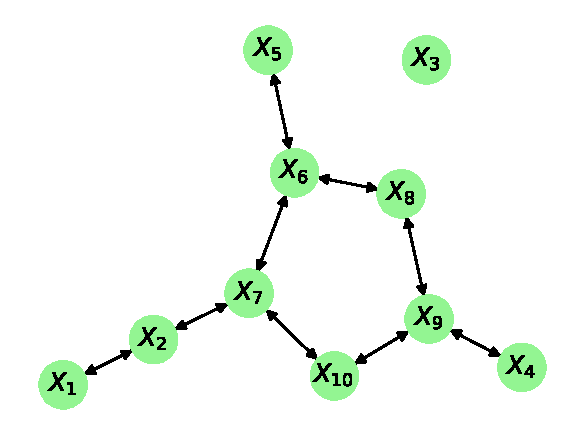
\includegraphics[width=.9\linewidth]{figures/Gaussian Network Theoretical/Graph from symmetric G obs - MI - cutoff 1_96e-2.pdf}
        \caption{$G_{dir}$ as a graph}
    \end{subfigure}
    \caption{Using a symmetric $G_{obs}$ instead of an upper triangular $G_{obs}$ result in near identical $G_{dir}$ in terms of relative weights on the edges. Namely, the $G_{dir}$ shown in (b) seem to be almost a scaled version of the (reflected) $G_{dir}$ derived from a triangular $G_{obs}$. Thus, as (c) also shows, we can accurately infer the structure of the network using a threshold $t = 1.96\cdot 10^{-2}$.}
    \label{fig:Gaussian network symmetric G_obs using mutual information}
\end{figure}

In conclusion, we observe a useful property of more general networks that for both mutual information and correlation, the additional assumption of the topological order does not have much of an effect in these cases contrary to what we observed for Gaussian chains and linear chain models in general, when using correlation.



\newpage


% \textcolor{red}{Example using Gaussian distribution and the error the algorithm makes.}


\section{CE computation}\label{sec:gaussian MI error}
Having discussed the strengths and weaknesses of \autoref{alg:ND}, we now turn our attention to \autoref{alg:Gobs1}. Namely, in this section we shall discuss the different methods from \autoref{subsec:Mutual information estimation and KDE methods} and how they perform on two examples. Once again, we shall base our results on two examples. The first is a simple case, where we shall see what to be aware of when initially the observations are transformed through estimated distribution functions as well as how accurate the different methods for estimating the Copula entropy i.e. mutual are. Continuing from the first example, we shall once again consider the network from \autoref{sec:General Gaussian graph} specified by \autoref{eq:example Gaussian network}. In particular, we will see how well the combined framework performs on an example we have already seen to be quite solvable if one uses accurate estimates of the mutual information which we previously calculated theoretically.



\subsection{Spline and KDE based CE estimation}
Before the first example, we shall discuss the problem with the spline based method and using histograms in general. Namely, we shall first see that if one were to just simply use a raw binning approach, the number of bins $N$ influences the estimate a lot and no number of bins seems to perform well on all cases. Namely, let $\boldsymbol X$ be a bivariate Gaussian with correlation $\rho$, then the Copula density looks as in \autoref{subfig:Gaussian copula density example}. In particular, we notice the peaks at $(0,0)$ and $(1,1)$ from which most of the mutual information originates. Now, simulating $n = 400$ observations from the joint distribution and transforming to the unit square through the marginal distribution function for varying correlations $\rho$, we can compare the estimated mutual information $I_{estim}$ using the results from \autoref{subsec:limit entropy and MI} to the true mutual information given by $ I_{exact} = - \frac{1}{2} \log \left(1 - \rho^2\right)$. The results are shown in \autoref{fig:raw histogram for MI estimation} where we report the relative size of the estimate and the exact mutual information and in \autoref{fig:raw hsitogram error for MI estimation} where the difference is reported. From \autoref{fig:raw histogram for MI estimation}, we might choose $N \approx 10$ as in \cite{Network-deconvolution-as-a-general-method-to-distinguish-direct-dependencies-in-networks} however for large correlations, we drastically underestimate mutual information. Increasing the number of bins to e.g. $N = 25$ corrects this error for large correlations, while small mutual information for small correlations remains relatively small. However, when deconvolving we would preferably want a more precise way of estimating the mutual information.

% but then small correlations have a relatively large error of around $0.5$ which is a relatively large error when comparing to the error the deconvolution step makes as illustrated in \autoref{fig:3 and 4 chain MI error}.

\begin{figure}[H]
    \centering
    \begin{subfigure}[t]{0.32\textwidth}
        \centering
        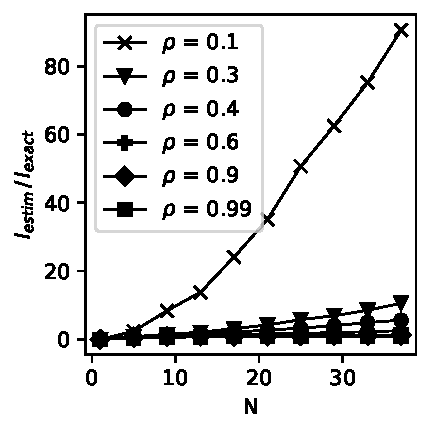
\includegraphics[width=\linewidth]{figures/ND examples/MI calc/gaussian example original all.pdf}
        \caption{}
        \label{subfig:d}
    \end{subfigure}%
    ~
    \begin{subfigure}[t]{0.32\textwidth}
        \centering
        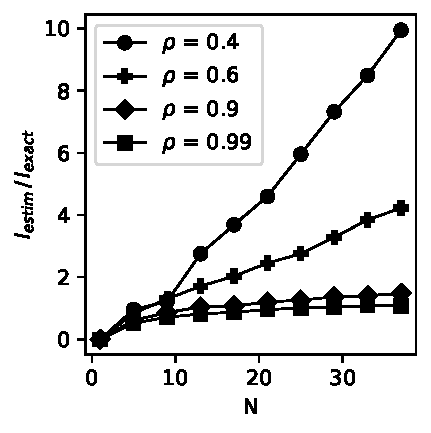
\includegraphics[width=\linewidth]{figures/ND examples/MI calc/gaussian example original zoom.pdf}
        \caption{}
        \label{subfig:dd}
    \end{subfigure}%
    ~
    \begin{subfigure}[t]{0.32\textwidth}
        \centering
        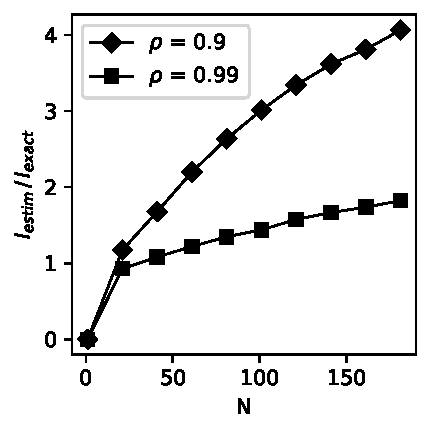
\includegraphics[width=\linewidth]{figures/ND examples/MI calc/gaussian example original high corr.pdf}
        \caption{}
        \label{subfig:ddd}
    \end{subfigure}
    \caption{Relative error when estimating mutual information for different bivariate Gaussian distributions with varying bin counts $N$. Information originating from small correlations are vastly overestimated.}
    \label{fig:raw histogram for MI estimation}
\end{figure}

\begin{figure}[H]
    \centering
    \begin{subfigure}[t]{0.4\textwidth}
        \centering
        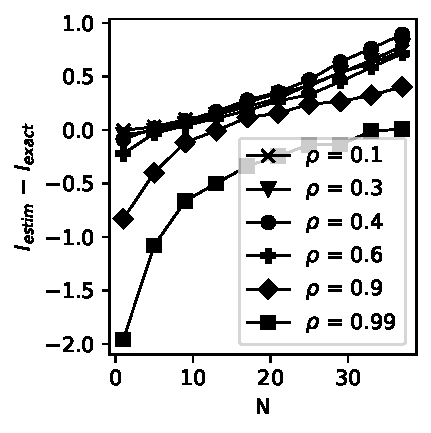
\includegraphics[width=\linewidth]{figures/ND examples/MI calc/gaussian example original all - error.pdf}
        \caption{}
        % \label{subfig:new MI method all}
    \end{subfigure}%
    ~
    \begin{subfigure}[t]{0.4\textwidth}
        \centering
        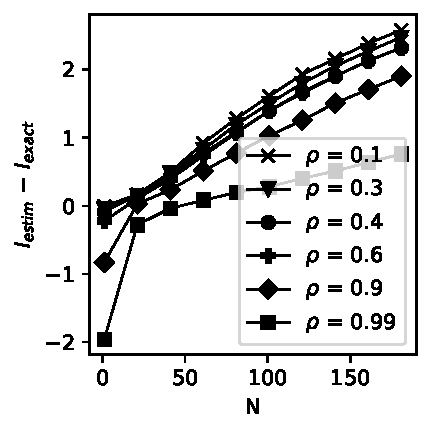
\includegraphics[width=\linewidth]{figures/ND examples/MI calc/gaussian example original all extended - error.pdf}
        \caption{}
        % \label{subfig:new MI method all zoom}
    \end{subfigure}
    \caption{Error for mutual information estimation for varying correlations. Contrary to the relative error, we see that it is the mutual information from larg ecorrlations that is the most error prone for small bin counts.}
    \label{fig:raw hsitogram error for MI estimation}
\end{figure}
We thus proceed with using the B-spline approach. Similar to the above results, in \autoref{fig:B-spline approach results MI - relative error} and \autoref{fig:B-spline approach results MI - error}, we observe that B-spline approach is prone to the same errors as the raw binning approach. However, from \autoref{fig:B-spline approach results MI - error} we see that the error are smaller for the B-spline based approach for large $N$ but also that a better choice for the number of bins is around $N = 50$ contrary to the results of \cite{Network-deconvolution-as-a-general-method-to-distinguish-direct-dependencies-in-networks}.


% med B-splines
\begin{figure}[H]
    \centering
    \begin{subfigure}[t]{0.32\textwidth}
        \centering
        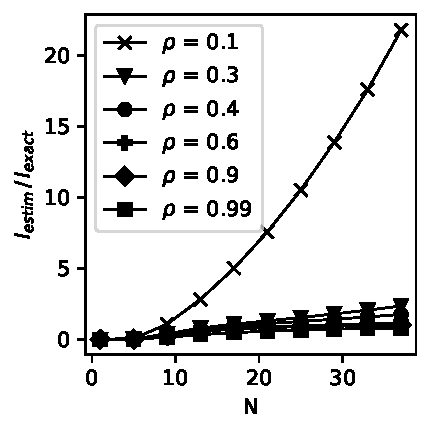
\includegraphics[width=\linewidth]{figures/ND examples/MI calc/gaussian example original all - B-spline.pdf}
        \caption{}
        % \label{subfig:d}
    \end{subfigure}%
    ~
    \begin{subfigure}[t]{0.32\textwidth}
        \centering
        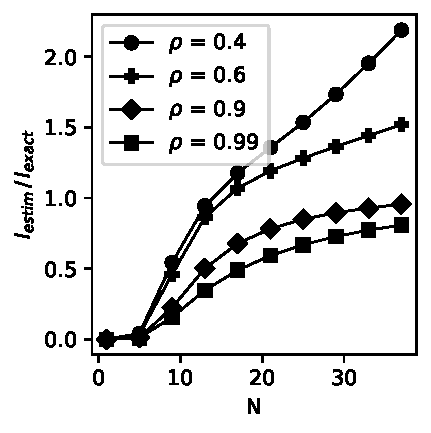
\includegraphics[width=\linewidth]{figures/ND examples/MI calc/gaussian example original high corr - B-spline.pdf}
        \caption{}
        % \label{subfig:dd}
    \end{subfigure}%
    ~
    \begin{subfigure}[t]{0.32\textwidth}
        \centering
        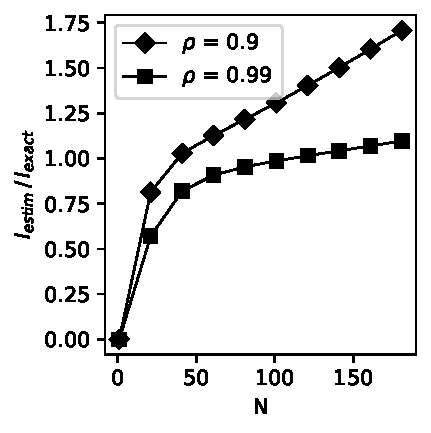
\includegraphics[width=\linewidth]{figures/ND examples/MI calc/gaussian example original zoom - B-spline.pdf}
        \caption{}
        % \label{subfig:ddd}
    \end{subfigure}
    \caption{Relative error of mutual information estimates using B-splines. Comparing to the relative error of the raw histogram based approach, we obtain relative error much smaller.}
    \label{fig:B-spline approach results MI - relative error}
\end{figure}

\begin{figure}[H]
    \centering
    \begin{subfigure}[t]{0.4\textwidth}
        \centering
        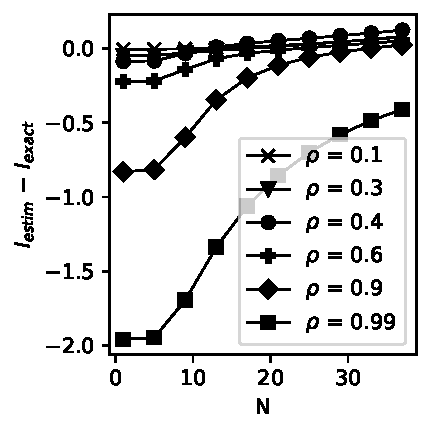
\includegraphics[width=\linewidth]{figures/ND examples/MI calc/gaussian example original zoom - B-spline - error.pdf}
        \caption{}
        % \label{subfig:new MI method all}
    \end{subfigure}%
    ~
    \begin{subfigure}[t]{0.4\textwidth}
        \centering
        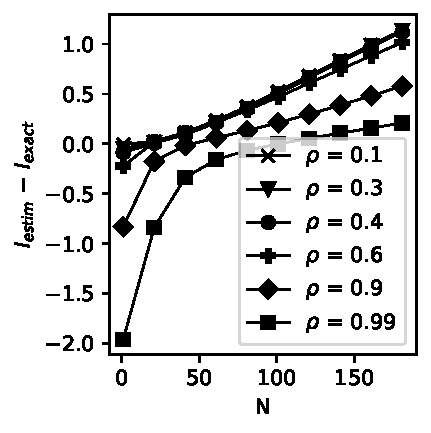
\includegraphics[width=\linewidth]{figures/ND examples/MI calc/gaussian example original high corr - B-spline - error.pdf}
        \caption{}
        % \label{subfig:new MI method all zoom}
    \end{subfigure}
    \caption{The actual error for mutual information estimation using the B-splines approach. For $n=400$ observations, performance is comparable to that of the raw histogram based approach although a larger bin count is preferred.}
    \label{fig:B-spline approach results MI - error}
\end{figure}
The results for M-splines are shown in \autoref{fig:M-spline approach results MI - error} and \autoref{fig:M-spline approach results MI - error} and we observe comparable performance except perhaps for a better estimation of mutual information for large correlations which is what we would expect from our discussion in \autoref{subsec:M-plines - method}.

The problem we observe with the above methods is that when mutual information is large, most of the mutual information comes from small domains at $(0,0)$ and $(1,1)$. Hence, to calculate the mutual information to a high precision, we need many bins. However, with many bins the estimate becomes more noisy as the support of each spline shrinks with $\frac{1}{N}$. However, as seen from \autoref{fig:approximation of mutual information knowing the true distribution}, if we can accurately estimate the Copula density function from observations, we can compute the mutual information perfectly by increasing the fineness of the integral approximation. In particular, the results below where obtained through the theoretical Copula density function evaluated at the bin centers $\left(\frac{2i - 1}{2N}, \frac{2j - 1}{2N}\right)$ for $i,j \in \{1,\dots, N\}$. We see that this simple approximation with $N = 1000$ is good for correlations up to $\rho = 0.99$. However, due to numerical limitations, we shall use $N = 500$ and only $n = 400$ observations to evaluate the performance of the KDE from the previous chapter. We note that a more memory efficient implementation is possible splitting up the computation in multiple parts as the problem with many observations and bins is that the computation is $\mathcal{O}\left(N^2n\right)$ time and memory if done all at once.
\begin{figure}[H]
    \centering
    \begin{subfigure}[t]{0.49\textwidth}
        \centering
        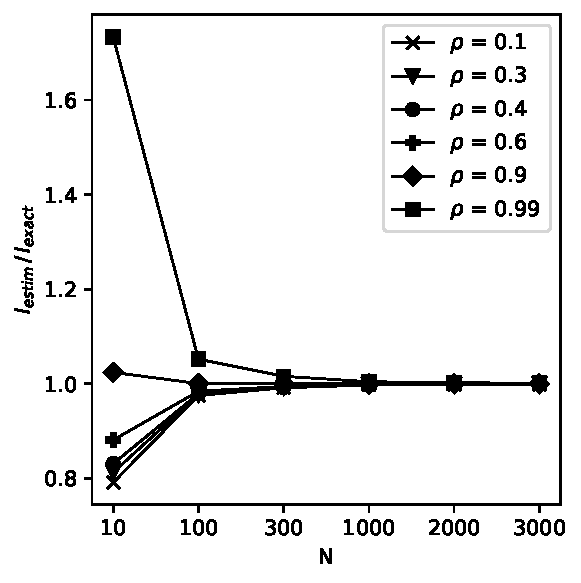
\includegraphics[width=\linewidth]{figures/ND examples/MI calc/gaussian example all.pdf}
        \caption{}
        \label{subfig:new MI method all}
    \end{subfigure}%
    ~
    \begin{subfigure}[t]{0.49\textwidth}
        \centering
        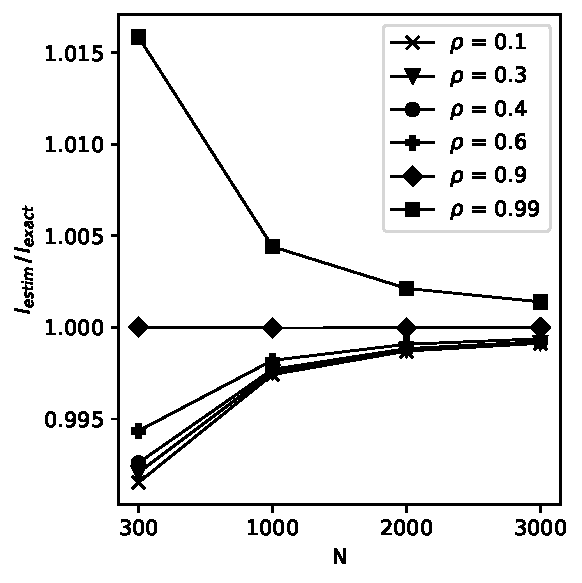
\includegraphics[width=\linewidth]{figures/ND examples/MI calc/gaussian example zoom.pdf}
        \caption{}
        \label{subfig:new MI method all zoom}
    \end{subfigure}
    \caption{Relative error of mutual information based on the true Copula density. We observe that for $N\geq 300$ the relative error is almost negligible.}
    \label{fig:approximation of mutual information knowing the true distribution}
\end{figure}




% rho 0.99 results - 1.9585177736258443 - 0.3 h_scott
% 1.6116888127939657
% 0.0010615687107130179

% rho 0.99 results - 1.9585177736258443
% 0.9510333150369028
% 0.00016328396291266664

% rho 0.9 results - 0.8303656034108255
% 0.6459377215632749
% 0.00044477897152890144

% rho 0.6 results - 0.22314355131420974
% 0.23094662195367777
% 0.0010027356448224958

% rho 0.4 results - 0.0871766935723889
% 0.09407501724301395
% 0.0003265470902529246

% rho 0.3 results - 0.047155339735620645
% 0.07017109137146779
% 0.0003795689303323563

% rho 0.1 results - 0.005025167926750725
% 0.02085490109213129
% 5.344562165818043e-05



In \autoref{tab:Jones error and variance}, we have used the boundary corrected KDE from \autoref{sec:Boundary corrected KDE} to first estimate the Copula density function and then estimate the mutual information from this. We note that by default, the bandwidth is chosen to be $h = h^{Scott} = 0.085$ as the marginals are approximately uniform and hence the variance is constant.
\begin{table}[ht]
    \centering
    \begin{tabular}{c|c|c|c}
        $\rho$ & $h$              & mean error  & variance                 \\\hline
        $0.1$  & $h^{Scott}$      & $ 0.01583$  & $5.3446 \cdot 10^{-5}$   \\
        $0.3$  & $h^{Scott}$      & $ 0.02302$  & $3.7957 \cdot 10^{-4}$   \\
        $0.4$  & $h^{Scott}$      & $ 0.006898$ & $3.2655  \cdot 10^{-4}$  \\
        $0.6$  & $h^{Scott}$      & $ 0.007803$ & $1.0027  \cdot 10^{-3}$  \\
        $0.9$  & $h^{Scott}$      & $-0.1844$   & $4.4478  \cdot 10^{-4} $ \\
        $0.99$ & $h^{Scott}$      & $-1.007$    & $1.6328  \cdot 10^{-4}$  \\
        $0.99$ & $0.3\,h^{Scott}$ & $-0.3468$   & $1.0616  \cdot 10^{-3}$
    \end{tabular}
    \caption{Estimating mutual information based on $n=400$ samples from different bivariate Gaussians using the boundary corrected KDE. Repeating the simulations $10$ times, we obtain average errors and variance of the estimate. In particular, the estimates are very certain for $n=400$. However, as for the spline based methods, large correlations result in underestimating the mutual information. This can however be corrected by tuning the bandwidth as is also observed in the above.}
    \label{tab:Jones error and variance}
\end{table}

From \autoref{tab:Jones error and variance}, we observe relatively low variance and in general, we compute the mutual information to a higher accuracy than either B-splines and M-splines. Thus, in the following example, we will only consider this method for estimating the mutual information between pairs of variables. In \autoref{fig:density estimate for Jones 1993 and theoretical copula rho 0.99} we have shown the estimated density and the theoretical copula. We observe that indeed the method accurately estimates the Copula density, although we note that the concept of a local bandwidth as discussed in \autoref{sec:Boundary corrected KDE} is likely to improve on the results as the peaks at $(0,0)$ and $(1,1)$ does not quite resemble those of the theoretical Copula density. In particular, we observe that reducing the bandwidth improves on the estimate. It is clearly observed by the improved resemblance with the theoretical Copula density. Although this is at the cost of undersmoothing on the interior. Indeed, a K-means based estimator of the bandwidth $h$ (as discussed in \autoref{sec:Boundary corrected KDE}) could work well as the mean distance near $(0,0)$ and $(1,1)$ is very small compared to the interior. However, we note that as long as observations are not close to perfectly correlated, the KDE based method performs quite well. This, we shall also see in the following section where we couple the above discussions on mutual information estimation with the deconvolution algorithm.
\newpage
\begin{figure}[H]
    \centering
    \begin{subfigure}[t]{0.49\textwidth}
        \centering
        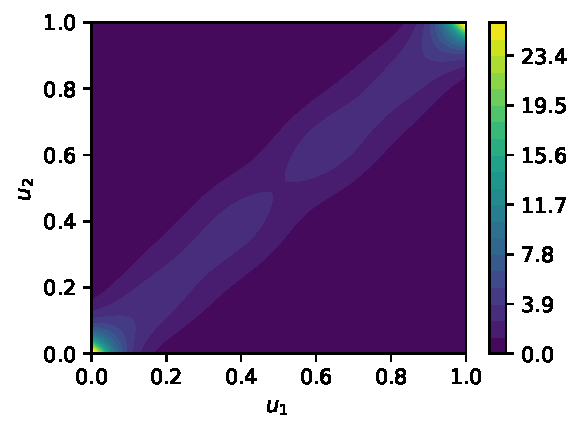
\includegraphics[width=\linewidth]{figures/MI estimation/regularized Jones - rho 0.99 - comparison of methods.pdf}
        \caption{}
        % \label{}
    \end{subfigure}
    \hfill
    \begin{subfigure}[t]{0.49\textwidth}
        \centering
        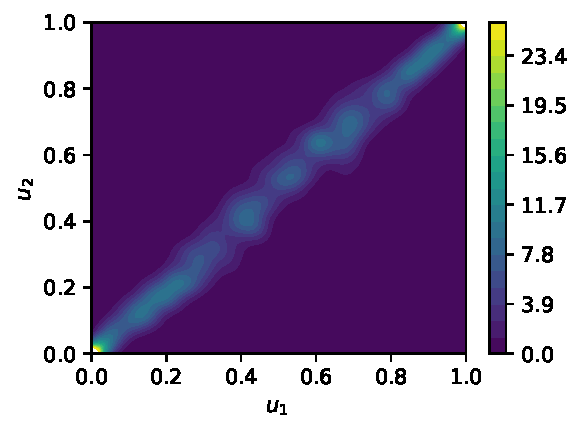
\includegraphics[width=\linewidth]{figures/MI estimation/regularized Jones - rho 0.99 - comparison of methods - 0.3 hscott.pdf}
        \caption{}
        % \label{}
    \end{subfigure}
    \\[\baselineskip]
    \begin{subfigure}[t]{0.49\textwidth}
        \centering
        \includegraphics[width=\linewidth]{figures/MI estimation/theoretical gaussian copula - rho 0.99 - comparison of methods.pdf}
        \caption{}
        \label{subfig:Gaussian copula density example}
    \end{subfigure}
    \caption{Estimated Copula densities (a) and (b) compared to the theoretical Copula density (c) for $\rho = 0.99$. Using a smaller bandwidth we are able to capture the peaks at $(0,0)$ and $(1,1)$ more accurately but at the cost of undersmoothing the interior.}
    \label{fig:density estimate for Jones 1993 and theoretical copula rho 0.99}
\end{figure}









\newpage
\subsection{Exponentiated multivariate Gaussian}\label{ex:1}
In this section, we will consider a small example, testing out the combined algorithm. In particular, we shall see what to be aware of when data is not easily transformed by the inverse distribution function. Let us consider a simple case with $\mathbf{Y} = e^{\mathbf{X}}$ (element wise exponentiation) where $X \sim \mathcal{N}\left(\mathbf{0}, \Sigma\right)$ where
$$\Sigma = \begin{bmatrix}
        \sigma_1^2           & 0.9\sigma_1\sigma_2 & 0          \\
        0.9 \sigma_1\sigma_2 & \sigma_2^2          & 0          \\
        0                    & 0                   & \sigma_3^2
    \end{bmatrix} = \text{diag}\left(\boldsymbol \sigma \right) \begin{bmatrix}
        1   & 0.9 & 0 \\
        0.9 & 1   & 0 \\
        0   & 0   & 1
    \end{bmatrix} \text{diag}\left(\boldsymbol \sigma \right)$$
In particular, in terms of \autoref{eq:Gaussian network in terms of Z}, we have that for $\boldsymbol X$, $\vec{\rho}_{1,2} = 0.9$. From \autoref{coro: Coordinate transformation}, it is clear that the (symmetric) mutual information matrix $G_{obs}$ is the same as of $boldsymbol X$ and hence by \autoref{prop:MI bivariate gaussian} is as follows
$$G_{obs} = \begin{bmatrix}
        0                                        & -\frac{1}{2} \log \left(1 - \vec{\rho}_{1,2}^2\right) & 0 \\
        \log \left(1 - \vec{\rho}_{1,2}^2\right) & 0                                                     & 0 \\
        0                                        & 0                                                     & 0
    \end{bmatrix} \approx \begin{bmatrix}
        0       & 0.83037 & 0 \\
        0.83037 & 0       & 0 \\
        0       & 0       & 0
    \end{bmatrix}$$
In particular, independent of the choice of $\boldsymbol \sigma$, we should observe an estimated $\hat{G}_{obs}$ close to this. We choose the following three cases for the choice of $\boldsymbol \sigma$.
$$
    \boldsymbol\sigma = (0.07, 0.3, 0.9), \quad
    \boldsymbol\sigma = (1,1,1), \quad
    \boldsymbol\sigma = (1,2,3)
$$

% It is clear that to \autoref{alg:Gobs1}, the mean of $\boldsymbol X$ is of no importance as it simply corresponds to a scaling of the $Y_i$ variables. Furthermore, because of \autoref{coro: Coordinate transformation}, theoretically, due to the uniqueness of the Copula $C$ (as $\boldsymbol Y$ is continuous) we should expect near equal or very similar results for $\boldsymbol Y$ and $\boldsymbol X$ from \autoref{alg:Gobs1}. Additionally, different $\boldsymbol \sigma$ corresponds to different scaling of $\boldsymbol X$, and thus we should observe equal or near equal $G_{dir}$ for all $\boldsymbol Y$ independently of $\boldsymbol \sigma$. Initially, we shall see how this hypothesis holds up when considering the following three examples

To draw from this distribution, one can either use built-in functions or use the Cholesky factorization of the correlation matrix to generate correlated variables from $3$ independent standard normal distributions and then scale with the chosen standard deviation to generate samples from all three cases based on the same seed. Once again, we shall only use $400$ samples as this resembles the number of observations in the pharmaceutical dataset, which we shall treat in \autoref{sec:Results - pharmaceutical data}. We note that a KDE has been used to approximate the distribution function. We will see in a moment why this is not always a good idea.


% In order for the sample size to not influence the results, we simulate a generous number of samples, namely, for the following results we have used $n = 10{,}000$ samples. 
For $\boldsymbol\sigma = (0.07, 0.3, 0.9)$, \autoref{alg:Gobs1} returns the following
\begin{equation} \label{eq:s small G_dir}
    \hat{G}_{obs} =
    \begin{bmatrix}
        0       & 0.8618  & 0.07889 \\
        0.8618  & 0       & 0.07880 \\
        0.07889 & 0.07880 & 0
    \end{bmatrix}
\end{equation}
% obs
% [0.        , 0.86179637, 0.07889214],
% [0.86179637, 0.        , 0.07879814],
% [0.07889214, 0.07879814, 0.        ]])

% dir
% [-0.32982227,  0.66018101,  0.03053256],
% [ 0.66018101, -0.32981569,  0.03042428],
% [ 0.03053256,  0.03042428, -0.00277444]

Similarly, for $\boldsymbol\sigma = (1,1,1)$:
\begin{equation} \label{eq:s medium G_dir}
    \hat{G}_{obs} =
    \begin{bmatrix}
        0      & 1.066  & 0.1667 \\
        1.066  & 0      & 0.1825 \\
        0.1667 & 0.1825 & 0
    \end{bmatrix}
\end{equation}
% obs
% [0.        , 1.06623794, 0.16669202],
% [1.06623794, 0.        , 0.18246652],
% [0.16669202, 0.18246652, 0.        ]]

% dir
% [-0.33102978,  0.65805331,  0.0474924 ],
% [ 0.65805331, -0.33263702,  0.06226742],
% [ 0.0474924 ,  0.06226742, -0.00899391]


Finally, for $\boldsymbol\sigma = (1,2,3)$:
$$ \hat{G}_{obs} =
    \begin{bmatrix}
        0      & 1.797 & 1.549 \\
        1.797  & 0     & 2.145 \\
        1.5492 & 2.145 & 0
    \end{bmatrix}
$$
% obs
% [[0.        , 1.79681262, 1.54927848],
% [1.79681262, 0.        , 2.14483483],
% [1.54927848, 2.14483483, 0.        ]

% dir
% [-3.29171674e-01,  6.60894478e-01,  1.71670151e-02],
% [ 6.60894478e-01, -3.29004287e-01,  1.12790451e-02],
% [ 1.71670151e-02,  1.12790451e-02, -6.14197155e-04]


Note that for this example, we have chosen $h = \frac{1}{3} h^{Scott}$ to correct for the behavior, observed in \autoref{tab:Jones error and variance}, when computing the mutual information between $X_1$ and $X_2$.

% The difference is likely produced by \autoref{alg:Gobs1} as if the resulting $G_{obs}$ was the same, then so would $G_{dir}$ and from the above argument, we know that theoretically this should be the case.

For $\boldsymbol\sigma = (0.07, 0.3, 0.9)$ we observe the most resemblance to the theoretical $G_{obs}$. For the latter two example,  $\boldsymbol\sigma = (1,1,1)$ and $\boldsymbol\sigma = (1,2,3)$, we see a completely different result and immediately suspect that there must be some errors either in the algorithm or the underlying assumptions of the algorithm. Investigating the partial results of \autoref{alg:Gobs1} we immediately see a flaw in the supposedly uniform variables $U_i$ as shown in figure \autoref{fig:Gaussian 3x3 large s uniforms} for $\boldsymbol\sigma = (1,2,3)$, which through a Kolmogorov Smirnov test are indeed significant (\autoref{tab:Results - 3x3 case - large s KS test}).
\begin{figure}[H]
    \centering
    \includegraphics[width=0.99\linewidth]{figures/ND examples/Gaussian 3x3 large s uniforms.pdf}
    \caption{The samples transformed using $U_i = F_i(Y_i)$ for $\boldsymbol\sigma = (1,2,3)$. These should be uniformly distributed, but clearly this is not the case for neither of them, as we have demonstrated in \autoref{tab:Results - 3x3 case - large s KS test}.}
    \label{fig:Gaussian 3x3 large s uniforms}
\end{figure}
\begin{table}[ht]
    \centering
    \begin{tabular}{c|c|c|c}
                & $U_1$   & $U_2$   & $U_3$   \\\hline
        $D_n$   & 0.16512 & 0.38354 & 0.42764 \\
        p-value & 0       & 0       & 0
    \end{tabular}
    \caption{Kolmogorov Smirnov test result based on 400 samples for $\boldsymbol\sigma = (1, 2, 3)$. It is clear that all samples are statistically significant.}
    \label{tab:Results - 3x3 case - large s KS test}
\end{table}


% Test-stat. :          0.16511676167616762
% Adjusted test-stat. : 3.3230573871137117
% p-value :             5.122165579629326e-10

% Test-stat. :          0.38353835383538354
% Adjusted test-stat. : 7.718901140114013
% p-value :             3.54203844926643e-52

% Test-stat. :          0.42764276427642767
% Adjusted test-stat. : 8.606524452445246
% p-value :             9.176555571039436e-65



Before handling this, the non-uniformity of $U_1$, $U_2$ and $U_3$ in \autoref{fig:Gaussian 3x3 large s uniforms} is likely also present in the case when $\boldsymbol\sigma = (1,1,1)$. Indeed, \autoref{fig:Gaussian 3x3 medium s uniforms} shows that this is indeed the case which is further shown significant in \autoref{tab:Results - 3x3 case - meadium s KS test}.
\begin{figure}[H]
    \centering
    \includegraphics[width=0.99\linewidth]{figures/ND examples/Gaussian 3x3 medium s uniforms.pdf}
    \caption{The samples transformed using $U_i = F_i(Y_i)$ for $\boldsymbol\sigma = (1,1,1)$.}
    \label{fig:Gaussian 3x3 medium s uniforms}
\end{figure}
\begin{table}[ht]
    \centering
    \begin{tabular}{c|c|c|c}
                & $U_1$   & $U_2$   & $U_3$                 \\\hline
        $D_n$   & 0.16511 & 0.14672 & 0.10561               \\
        p-value & 0       & 0       & $2.382 \cdot 10^{-4}$
    \end{tabular}
    \caption{Kolmogorov Smirnov test result based on 400 samples for $\boldsymbol\sigma = (1, 1, 1)$. Once again, all of the transformed samples are shown shown statistically significant.}
    \label{tab:Results - 3x3 case - meadium s KS test}
\end{table}

% Test-stat. :          0.16511676167616762
% Adjusted test-stat. : 3.3230573871137117
% p-value :             5.122165579629326e-10

% Test-stat. :          0.14671542154215422
% Adjusted test-stat. : 2.952721216246625
% p-value :             5.347893594719433e-08

% Test-stat. :          0.1056125612561256
% Adjusted test-stat. : 2.125505601560156
% p-value :             0.00023819975157518748


Finally, for the sake of completeness, $\boldsymbol\sigma = (0.07, 0.3, 0.9)$ is also shown in \autoref{fig:Gaussian 3x3 small s uniforms} and seems very reasonable, except for $U_3$ which again, is shown through the Kolmogorov Smirnov test in \autoref{tab:Results - 3x3 case - small s KS test} to be significant.
\begin{figure}[H]
    \centering
    \includegraphics[width=0.99\linewidth]{figures/ND examples/Gaussian 3x3 small s uniforms.pdf}
    \caption{\raggedright The samples transformed using $U_i = F_i(Y_i)$ for $\boldsymbol\sigma = (0.07, 0.3, 0.9)$.\hfill}
    \label{fig:Gaussian 3x3 small s uniforms}
\end{figure}
\begin{table}[ht]
    \centering
    \begin{tabular}{c|c|c|c}
                & $U_1$    & $U_2$    & $U_3$     \\\hline
        $D_n$   & 0.029036 & 0.029026 & 0.085611  \\
        p-value & 0.88427  & 0.88454  & 0.0052791
    \end{tabular}
    \caption{Kolmogorov Smirnov test result based on 400 samples for $\boldsymbol\sigma = (0.07, 0.3, 0.9)$.}
    \label{tab:Results - 3x3 case - small s KS test}
\end{table}

% Test-stat. :          0.029036403640364084
% Adjusted test-stat. : 0.5843721414641474
% p-value :             0.8842745431056299

% Test-stat. :          0.029025652565256466
% Adjusted test-stat. : 0.584155770702069
% p-value :             0.8845411493088176

% Test-stat. :          0.08561056105610561
% Adjusted test-stat. : 1.7229553465346537
% p-value :             0.005279081841001786


From the above examples, it seems that the larger the variance, the worse the uniforms turn out. From \autoref{fig:Gaussian 3x3 large s X3 KDE}, we see that this is primarily due to a poor fit of the KDE, where we have zoomed in on the interval $[-200 , 200]$ which contains $96.2\%$ of observations. In particular, the peak neat $y_3 = 0$ is not captured by the KDE. The poor fit is primarily due to the use of Scott's Rule which in this case overshoots the optimal bandwidth by a lot. The poor fit also explains the high concentration of $U_3$ around $0.5$ in \autoref{fig:Gaussian 3x3 large s uniforms} as only $54.5\%$ of the probability mass for the KDE lies above $0$.
\begin{figure}[ht]
    \centering
    \includegraphics[width=0.7\linewidth]{figures/ND examples/Gaussian 3x3 large s X3 KDE.pdf}
    \caption{Inspecting the fit of the KDE on $Y_3$, we indeed observe that it is quite poor. The peak near $0$ is not captured. Thus, either $Y_3$ has to be transformed through some strictly positive function or another estimate of the distribution function (such as the empirical distribution function) need to be applied.}
    \label{fig:Gaussian 3x3 large s X3 KDE}
\end{figure}

By \autoref{coro: Coordinate transformation}, we can get rid of this numerical issues by transforming $Y_i$ using e.g. $\log(\cdot)$ or $(\cdot)^{p}$ for $p>0$ to even out the observations more. As the first simply inverts the initial transformation of $\boldsymbol X$, we choose the latter as a more interesting case. In particular, choosing $p<1$ will result in a more even distribution. In the following, $p=1/10$ has been used to transform $\boldsymbol Y$, resulting in $\boldsymbol Y^p$, prior to running \autoref{alg:Gobs1}. The resulting samples $u_i^{(j)}$ are shown in \autoref{fig:Gaussian 3x3 large s power uniforms} along with statistical test for uniform distribution in \autoref{tab:Results - 3x3 case - large s KS test - transformed}


% Test-stat. :          0.029436443644364485
% Adjusted test-stat. : 0.5924231465646576
% p-value :             0.8741535027574947

% Test-stat. :          0.028525602560255936
% Adjusted test-stat. : 0.5740920143264309
% p-value :             0.8966183595247508

% Test-stat. :          0.028819631963196313
% Adjusted test-stat. : 0.5800095030753074
% p-value :             0.8895941793129514

The resulting $u_i^{(j)}$ are now no longer significant and indeed the KDE fits much better as seen in \autoref{fig:Gaussian 3x3 large s power X3 KDE}. Furthermore, the estimated $\hat{G}_{obs}$ in \autoref{eq:G_obs hat power transformed Y - 3x3} is similar to the one obtained from $\boldsymbol \sigma = \left(0.07,\, 0.3,\, 0.9\right)$ with the notable difference $I(Y_1,Y_3)$ and $I(Y_2,Y_3)$ are closer to the true value, $0$.
\begin{figure}[ht]
    \centering
    \includegraphics[width=0.99\linewidth]{figures/ND examples/Gaussian 3x3 large s power uniforms.pdf}
    \caption{The resulting observations of $\boldsymbol U$ after a power transformation with $p = 1/10$ has been applied to $\boldsymbol Y$.}
    \label{fig:Gaussian 3x3 large s power uniforms}
\end{figure}
\begin{table}[ht]
    \centering
    \begin{tabular}{c|c|c|c}
                & $U_1$     & $U_2$     & $U_3$     \\\hline
        $D_n$   & 0.0061099 & 0.0061435 & 0.0073148 \\
        p-value & 0.84838   & 0.84368   & 0.65690
    \end{tabular}
    \caption{Based on 400 samples of $\boldsymbol Y^p $ with $\boldsymbol\sigma = (1, 2, 3)$ neither are statistically significant.}
    \label{tab:Results - 3x3 case - large s KS test - transformed}
\end{table}

\begin{figure}[H]
    \centering
    \includegraphics[width=0.7\linewidth]{figures/ND examples/Gaussian 3x3 large s power X3 KDE.pdf}
    \caption{The KDE fit on $Y_3^p$ with $p = 1/10$. Now, the KDE fits the samples much better, leading to non-significant results regarding tests of uniformity.}
    \label{fig:Gaussian 3x3 large s power X3 KDE}
\end{figure}

\begin{equation}\label{eq:G_obs hat power transformed Y - 3x3}
    \hat{G}_{obs} = \begin{bmatrix}
        0       & 0.8629  & 0.01799 \\
        0.8629  & 0       & 0.01886 \\
        0.01799 & 0.01886 & 0
    \end{bmatrix}
\end{equation}
% [0.        , 0.86287956, 0.01798837],
% [0.86287956, 0.        , 0.01886115],
% [0.01798837, 0.01886115, 0.        ]

% Turning to \autoref{alg:Gobs1} and \autoref{alg:ND} we now find that $G_{dir}$ is given by
% $$G_{dir} =
%     \begin{bmatrix}
%         -0.3290 & 0.6610   & 0.01188    \\
%         0.6610  & -0.3289  & 0.004603   \\
%         0.01188 & 0.004603 & -0.0002167
%     \end{bmatrix}
% $$

% [-3.29010102e-01,  6.61023097e-01,  118799447e-02],
% [ 6.61023097e-01, -3.28890183e-01,  4.60309150e-03],
% [ 1.18799447e-02,  4.60309150e-03, -2.16682793e-04]



Which is indeed much more comparable with the result from before in \autoref{eq:s medium G_dir} and \autoref{eq:s small G_dir}. The difference between $G_{dir}$ from $\boldsymbol Y$ and $\boldsymbol Y^p$ is clearly visible in \autoref{fig:Gaussian 3x3 large s G_dir differences} and also \autoref{fig:Gaussian 3x3 large s power} resembles the original correlation structure.
\begin{figure}[H]
    \centering
    \begin{subfigure}[t]{0.49\textwidth}
        \centering
        \includegraphics[width=\linewidth]{figures/ND examples/Gaussian 3x3 large s.pdf}
        \caption{}
        \label{fig:Gaussian 3x3 large s}
    \end{subfigure}%
    ~
    \begin{subfigure}[t]{0.49\textwidth}
        \centering
        \includegraphics[width=\linewidth]{figures/ND examples/Gaussian 3x3 large s power.pdf}
        \caption{}
        \label{fig:Gaussian 3x3 large s power}
    \end{subfigure}
    \caption{$G_{dir}$ resulting from $400$ samples from multi variate Gaussian with $\boldsymbol\sigma = (1,2,3)$ in \textbf{(a)} with raw samples from $\boldsymbol Y$ and in \textbf{(b)} the transformed data corresponding to $\boldsymbol Y^p$.}
    \label{fig:Gaussian 3x3 large s G_dir differences}
\end{figure}
Finally, to end this example we shall compare with some theoretical results. Namely, the output $G_{obs}$ of \autoref{alg:Gobs1} can also be calculated theoretically. For this, we shall use \autoref{prop:MI bivariate gaussian} which permits a theoretical result, namely
\begin{align*}
    G_{obs} & =
    \begin{bmatrix}
        0                                              & -\frac{1}{2} \ln \left( 1 - \rho_{12}^2\right) & -\frac{1}{2} \ln \left( 1 - \rho_{13}^2\right) \\
        -\frac{1}{2} \ln \left( 1 - \rho_{21}^2\right) & 0                                              & -\frac{1}{2} \ln \left( 1 - \rho_{23}^2\right) \\
        -\frac{1}{2} \ln \left( 1 - \rho_{31}^2\right) & -\frac{1}{2} \ln \left( 1 - \rho_{32}^2\right) & 0
    \end{bmatrix} \\
            & \cong
    \begin{bmatrix}
        0       & 0.83037 & 0 \\
        0.83037 & 0       & 0 \\
        0       & 0       & 0
    \end{bmatrix}
\end{align*}
Similarly, prior to deconvolution, using just the sampled $\boldsymbol X$ (i.e. no exponential transform), \autoref{alg:Gobs1} returns
$$G_{obs} =
    \begin{bmatrix}
        0.         & 0.64069542 & 0.01824538 \\
        0.64069542 & 0.         & 0.0135368  \\
        0.01824538 & 0.0135368  & 0.
    \end{bmatrix}
$$

If we adjust the algorithm to account for the non-unifority, it works well even with sigma 3


% \textcolor{red}{Test om denne G er lige den teoretiske. Eller nærmere, argumenter for hvorfor vi ikke laver en test, eller hvad man kunne gøre. Har samplet fra en simultan normalfordeling, så kan lave en til en mellem MI og korrelation. }

% From the confidence density for the correlation $\rho$ given the emperical correlation $r$ is given by
% $$f\left(\rho \mid r,\nu\right) = \frac{\nu (\nu-1) \Gamma(\nu-1)}{\sqrt{2\pi} \Gamma(\nu + \frac{1}{2})} \frac{\left(1-r^2\right)^{\frac{\nu-1}{2}} \left(1-\rho^2\right)^{\frac{\nu-2}{2}} }{\left(1-r\rho\right)^{\frac{2\nu-1}{2}}} F\left(\frac{3}{2}, -\frac{1}{2}, \nu+\frac{1}{2}, \frac{1+r\rho}{2}\right)$$
% from the mutual information, we can calculate the absolute correlation. Notice that the density does not change when reversing both $r$ and $\rho$ simultaneously, thus, without loss of generality, assume $r\geq 0$, then we can calculate a CI for $\rho$ (which will be negated if we had used $-r$ instead and thus would be identical when taking the absolute value). If the original CI $[a,b]$ contains $0$ i.e. $a<0$, we shall write the CI for the absolute correlation as $[0,b]$ instead. This way, we can compare the absolute correlations and see if they are the same (by checking if the CI contains the theoretical correlation) by \cite{Confidence_in_Correlation}. Using numerical integration (fast enough with high numerical accuracy from many bins, 1 mil bins, yielding probability mass 1.0000000000008133), can compute CI for absolute correlation

\autoref{sec:bivar gauss abs correlation CI}


Clearly these are not equal, but in this case, the error is suspected to originate from the estimated joint density. For example, considering $X_1$ and $X_2$, we compare the estimated joint copula density and compare to the theoretical \textcolor{red}{reference til et sted hvor gausisk copula står} shown in \autoref{fig:gaussian copula estimate} and \autoref{fig:gaussian copula truth} respectively.
\begin{figure}[H]
    \centering
    \begin{subfigure}[t]{0.45\linewidth}
        \centering
        \includegraphics[width = \linewidth]{figures/ND examples/Gaussian copula sample contour.pdf}
        \caption{}
    \end{subfigure}%
    ~
    \begin{subfigure}[t]{0.5\linewidth}
        \includegraphics[width = \linewidth]{figures/ND examples/Gaussian copula sample pdf.pdf}
        \caption{}
    \end{subfigure}
    \caption{Estimated copula density $c$ with $\rho = 0.9$ corresponding to $X_1$ and $X_2$.}
    \label{fig:gaussian copula estimate}
\end{figure}
The noticeable difference is in the corners $(0,0)$ and $(1,1)$ where the theoretical copula density tends to infinity whereas the estimated density has modes at $(0.1,0.1)$ and $(0.9,0.9)$. In particular, simply rescaling the copula density in \autoref{alg:Gobs1} does not resemble the theoretical boundary which is a known issue \textcolor{red}{reference til artikel om undershoot peaks og boundary conditions for KDE}. A better approach may be to use jackknifing \textcolor{red}{link til afsnit of jackknifing, som også indeholder reference til artikel hvor dette gøres}.
\begin{figure}[H]
    \centering
    \begin{subfigure}[t]{0.49\linewidth}
        \centering
        \includegraphics[width = \linewidth]{figures/ND examples/Gaussian copula theoretical contour.pdf}
        \caption{}
    \end{subfigure}%
    ~
    \begin{subfigure}[t]{0.49\linewidth}
        \includegraphics[width = \linewidth]{figures/ND examples/Gaussian copula theoretical pdf.pdf}
        \caption{}
    \end{subfigure}
    \caption{Theoretical copula density $c$ with $\rho = 0.9$ corresponding to $X_1$ and $X_2$.}
    \label{fig:gaussian copula truth}
\end{figure}
We note however, that the underlying structure is still captured i.e. that $Y_1$ and $Y_2$ covary while $Y_3$ does not inform $Y_1$ or $Y_2$ and vice versa.


We continue with a similar example to the previous one. The key difference is the number of variables and a more complicated correlation structure to test the algorithms further.



\newpage

% Future works:
%  - undersøg K-means og adaptive bandwidth for mere præcise estimater af MI
%  - Brug den inferrede causale struktur til at lave inferens og hvor godt den holde op mod observeerede data - E.g. PyBanshee, som er et ikke parametrisk bayesians networks
%  - Undersøg flere mål for association såsom partial correlation, generalization of mutual information that are directed (f.eks. er der intuitivt mere information fra X1 -> X2 hvis X2 = f(X1) men ikke den anden vej), x2y (ability of x to predict y)


\subsection{Gaussian network revisited - Application of complete framework}\label{sec:Gaussian network MI example - computation}
In this section, we will redo the example from \autoref{sec:General Gaussian graph} where the underlying causal structure was defined in \autoref{eq:example Gaussian network}. However, this time, we shall first simulate $n = 400$ observations from the joint distribution and then estimate the Copula density based on these observations instead of using the theoretical Copula densities (i.e. the exact mutual information) along with the learnings from the previous sections. In particular, we shall observe that the algorithm for estimating the mutual information between pairs of the random variables performs well enough for us to recover the structure perfectly. As the largest (direct) correlation is $0.7$, we expect from \autoref{tab:Jones error and variance} that the mutual information will be accurately estimated.


% None are significant (marginal distribution).


% For $10$ variables, took around 25 mintues



In \autoref{fig:estimated MI 10 Gaussian results}, we have summarized the results using a symmetric $G_{obs}$. In particular, we observe that the estimated $\hat{G}_{dir}$ is nearly identical to the true $G_{dir}$ (from \autoref{eq:example Gaussian network}). In particular, choosing the relatively small threshold $t = 0.06$ we recover the true causal structure although the entries of $\hat{G}_{dir}$ appear to be a factor $2$ as large as the true $G_{dir}$. If we instead assume a topological structure, resulting in a triangular $\hat{G}_{obs}$, this deviation is alleviated as seen in \autoref{fig:estimated MI 10 Gaussian results - triangular}.

From this short example on combining \autoref{alg:Gobs1} and \autoref{alg:ND}, we observe that indeed the methodology proposed can at least for networks as defined in \autoref{sec:General Gaussian graph} recover the causal structure. Furthermore, from \autoref{coro: Coordinate transformation}, we note that the same structure would be inferred if instead the variables had been transformed by a strictly increasing function. This is particularly important in the following section where we shall use the framework on the data introduced in \autoref{chap:data}.

As an example, suppose that a network is defined as in \autoref{sec:General Gaussian graph}, but we only observe $\boldsymbol Y$ where $Y_i = f \left(X_i\right)$ with $f$ being strictly positive. Then, the mutual information between $Y_i$ and $Y_j$ is the same as between $X_i$ and $X_j$ which we from this example is accurately deconvolved.

\newpage
\begin{figure}[H]
    \centering
    \begin{subfigure}[t]{0.49\linewidth}
        \includegraphics[width = \linewidth]{figures/ND examples/Gaussian network 10 - G_dir - symmetric.pdf}
        \caption{$\hat{G}_{dir}$}
    \end{subfigure}
    \hfill
    \begin{subfigure}[t]{0.49\linewidth}
        \includegraphics[width = \linewidth]{figures/ND examples/Gaussian network 10 - G_dir true - symmetric.pdf}
        \caption{$G_{dir}$}
    \end{subfigure}
    \\[\baselineskip]
    \begin{subfigure}[t]{0.49\linewidth}
        \includegraphics[width = \linewidth]{figures/ND examples/Gaussian network 10 - G_dir as graph - symmetric.pdf}
        \caption{$\hat{G}_{dir}$ as a graph}
    \end{subfigure}
    \caption{Combining the method for estimating the mutual information and algorithm for deconvolving the network (using a symmetric $G_{obs}$) we observe near optimal results. In particular, the structure of $\hat{G}_{dir}$ (a) is very alike to $\hat{G}_{dir}$ (b). This is also shown in (c), where the $\hat{G}_{dir}$ is represented as a graph using $t = 0.06$, and we recover the original graphical structure. We do however observe that the entries of $\hat{G}_{dir}$ are almost twice the size of $G_{dir}$.}
    \label{fig:estimated MI 10 Gaussian results}
\end{figure}

\newpage
\begin{figure}[H]
    \centering
    \begin{subfigure}[t]{0.49\linewidth}
        \includegraphics[width = \linewidth]{figures/ND examples/Gaussian network 10 - G_dir - triangular.pdf}
        \caption{$\hat{G}_{dir}$}
    \end{subfigure}
    \hfill
    \begin{subfigure}[t]{0.49\linewidth}
        \includegraphics[width = \linewidth]{figures/ND examples/Gaussian network 10 - G_dir true - triangular.pdf}
        \caption{$G_{dir}$}
    \end{subfigure}
    \\[\baselineskip]
    \begin{subfigure}[t]{0.49\linewidth}
        \includegraphics[width = \linewidth]{figures/ND examples/Gaussian network 10 - G_dir as graph - triangular.pdf}
        \caption{$\hat{G}_{dir}$ as a digraph}
    \end{subfigure}
    \caption{When assuming a topological order of the random variables, we observe that the inferred $\hat{G}_{dir}$ (a) is much more alike the true $G_{dir}$ (b). Furthermore, using a threshold $t = 0.05$ we recover the true causal structure, removing the noise entries in $\hat{G}_{dir}$.}
    \label{fig:estimated MI 10 Gaussian results - triangular}
\end{figure}

% \textcolor{red}{casuality svarer til at lave nedre/øvre trekant. Er der forskel i at gør edet før og efter for en symmetrisk matrix? - Ja, men begge metoder på 10 eksempel giver gode resultater. Kommenter at det er matematisk meget forskelligt at filtrere først og så ND efter og omvendt}



\newpage
\section{Pharmaceutical data deconvolution}\autoref{sec:Results - pharmaceutical data}
Finally, we turn our attention to the pharmaceutical production data introduced in \autoref{chap:data}. Namely, we have at this point used the methodology discussed in \autoref{chap:results} both to estimate mutual information, to deconvolve Gaussian networks and chains based on analytical expressions for the correlation between variables and finally in \autoref{sec:Gaussian network MI example - computation} where we have combined \autoref{alg:Gobs1} and \autoref{alg:ND} to infer the causal structure of a $10$-dimensional Gaussian network.

In particular, we saw that the methodology combined produced very accurate results when the mutual information between pairs of random variables were not too large as these proved difficult to estimate to high accuracy without turning to a manual tuning of the bandwidths. We especially want to avoid the manual tuning of the bandwidth in this section, as we shall compute mutual information between $1653$ pairs of random variables.

The random variables are the duration and delays of each process as well as the change in level of the tank during these operations. Recall that e.g. $T^P_{4.1}$ is the duration of process $4.1$ while $T^D_{4}$ is the delay after all subprocesses of process $4$ are completed. Also, for each \textit{temporal} variable $T^P_i$ and $T^D_i$, we have a corresponding change of level $M^P_i$ and $M^D_i$. Initially, we also add the accumulated random variables. Namely, for process $1$, we add the random variable $T_1 = T^P_1 + T^D_1$ and likewise for the level changes for all processes. Also, the total duration $T = \sum_{i=1}^{10} T_i$ and change in level $M = \sum_{i=1}^{10} M_i$ are added as random variables. The accumulated random variables are initially added to see if our method can \textit{rediscover} these simple causal relations. We will later remove these from our discussion as we try to gain a deeper understanding of the production system.

Hence, from the above, we initially have $68$ variables. However, some of them are constant and thus out of interest. The constant \textit{random} variables are
$$M^D_1,\quad  M^D_2,\quad T^P_{4.1},\quad  M^P_{4.1},\quad T^P_{4.3},\quad  M^D_4,\quad  M^D_6,\quad  T^P_8,\quad  M^D_{10}$$
However, as $T_8 = T^P_8 + T^D_8$ we shall also exclude either $T_8$ or $T^D_8$ due to $T^P_8$ being constant. In particular, $T_8$ and $T^D_8$ can be interchanged at will when computing mutual information according to \autoref{coro: Coordinate transformation}. Here, we have chosen to keep $T^D_8$ as it is easier to relate to the other processes. Thus, we are only considering $58$ random variables and hence $58 \cdot 57 / 2 = 1653$ pairs of variables as stated above.

We note that as the resolution in time is $0.001$ we add uniform distributed noise from $[0,0.001]$ to the durations and delays. In particular, we observe that in some cases equal durations are observed. These would result in non-uniform marginals like in \autoref{ex:1} hence making the algorithm fail at computing the mutual information accurately. We note that the experiments to follow have been carried out multiple times to assess the influence of this perturbation to the durations and delays. However, as this did not influence our results in the slightest we will not discuss this further. Furthermore, instead of using a KDE as in \autoref{ex:1} to transform the (continuous) observations to lie on the unit interval through the distribution function, we have used the empirical distribution function. This was done to ensure that all $58$ random variables were transformed appropriately without having to consider transformations (like in \autoref{ex:1}).

\begin{figure}[ht]
    \centering
    \includegraphics[width = .9\linewidth]{figures/Cycle data/G_dir complete - symmetric.pdf}
    \caption{$G_{dir}$ from a symmetric $G_{obs}$. Other than the accumulated variables, we observe strong dependencies between the duration of a process and the change in level during the process by comparing the columns and rows labeled $T^P_i$ and $M^P_i$.}
    \label{fig:Cycle data - G_dir all}
\end{figure}

The resulting $G_{obs}$ is shown in the appendix, \autoref{fig:Cycle data - G_obs all}. We observe that there indeed is a strong dependence between the accumulated variables and their summands such as $T_1$ and $T^D_1$ as well as $T^P_1$. We immediately use the deconvolution algorithm resulting in the $G_{dir}$ seen in \autoref{fig:Cycle data - G_dir all}


We have labeled sections of $G_{dir}$ such that each sections corresponds to and ordered list of variables. The variables in each section are
\begin{equation}\label{eq:Cycle data sets of variables}
    \begin{aligned}
        T_i^D & = \left\{ T^D_1, T^D_2, T^D_3, T^D_4, T^D_5, T^D_6, T^D_7, T^D_8, T^D_9, T^D_{10} \right\}                                 \\
        T^P_i & = \left\{ T^P_1, T^P_2, T^P_{3.1}, T^P_{3.2}, T^P_{4.2}, T^P_{5}, T^P_{6}, T^P_{7}, T^P_9, T^P_{10}\right\}                \\
        T_i   & = \left\{T_1, T_2, T_3, T_4, T_5, T_6, T_7, T_9, T_{10}\right\}                                                            \\
        T     & = \left\{T\right\}                                                                                                         \\
        M^D_i & = \left\{ M^D_3, M^D_5, M^D_7, M^D_8, M^D_9 \right\}                                                                       \\
        M^P_i & = \left\{ M^P_1, M^P_2, M^P_{3.1}, M^P_{3.2}, M^P_{4.2}, M^P_{4.3}, M^P_{5}, M^P_6, M^P_7, M^P_8, M^P_9, M^P_{10} \right\} \\
        M_i   & = \left\{M_1, M_2, M_3, M_4, M_5, M_6, M_7, M_8, M_9, M_{10}\right\}                                                       \\
        M     & = \left\{M\right\}
    \end{aligned}
\end{equation}

I.e. the section labeled $T^D_i$ consists of all the delays after each process and so on for the remaining section labels.


From \autoref{fig:Cycle data - G_dir all}, we observe that the accumulated durations of each process $T_i$ is indeed very dependent on both the delay and durations of the process. This is a sign that the algorithm performs well as by definition $T_i = T^D_i + \sum_{k\in \mathcal{P}_i} T^P_i$ (where $\mathcal{P}_i$ is defined as the set of subprocesses that constitute the process $i$).
\begin{figure}[H]
    \centering
    \begin{subfigure}[t]{0.49\linewidth}
        \includegraphics[width = .9\linewidth]{figures/Cycle data/G_dir complete - symmetric - TD4 vs T4.pdf}
        \caption{}
    \end{subfigure}
    \hfill
    \begin{subfigure}[t]{0.49\linewidth}
        \includegraphics[width = .9\linewidth]{figures/Cycle data/G_dir complete - symmetric - TP4 vs T4.pdf}
        \caption{}
    \end{subfigure}
    \caption{$T_4$ vs $T^D_4$ and $T^P_{4.2}$ in (a) and (b) respectively. Notice that the continuous part of the variables has been transformed using the empirical distribution function such that the domain is $[0,1]$ for all the variables. The transformation allows for an easier assessment of the mutual information between the pairs of variables.}
    \label{fig:T4 vs TD4 and TP4.2}
\end{figure}

For example, we observe that $T^D_4$ is strongly associated with $T_4$ while $T^P_{4.2}$ is not as strongly associated with $T_4$. However, there is still a connection. If we plot $T_4$ vs. $T^D_4$ and $T^P_{4.2}$ respectively (\autoref{fig:T4 vs TD4 and TP4.2}) we indeed observe that the information between $T^D_4$ and $T_4$ is much greater than $T^P_{4.2}$ and $T_4$. As we saw in \autoref{chap:data}, this is because the delays after process $4$ are much larger than the duration to begin with. Thus, even though $T^D_4$ is $0$, $56.25\%$ of times, most of $T_4$ can be explained from this alone, when comparing to the scores between $T_4$ and the other random variables.

Furthermore, we observe that the total duration $T$ is mostly explained by $T_7$ which in turn is explained mostly by $T^P_7$. Although there are many other interesting observations such as the most change in levels and masses occurs during process $3$, addition of a material and stirring. The level after process $3$ is in turn mostly influenced by the stirring but also seem to have some unexplained variation. We observe the unexplained variation from the row corresponding to $M_3$ which has relatively small associations with the other delays, durations and levels.

At this point, we have observed that the algorithm rediscovers what we already know to be true. Namely, that the total masses and process durations are well explained by the individual processes. However, a more interesting question is how each of the processes affect each other. More precisely, if we only consider each process without the accumulated random variables $T_i$, $T$, $M_i$ and $M$, we hope to discover more interesting dependencies between the processes. Also, $T_i$ etc. can always be computed from the processes, so we do not really care for these random variables if we want to understand the dynamics of the system.

\begin{figure}[ht]
    \centering
    \begin{subfigure}[t]{0.49\linewidth}
        \includegraphics[width = \linewidth]{figures/Cycle data/G_dir times - symmetric.pdf}
        \caption{$G_{dir}$}
        \label{subfig:G_dir using only times}
    \end{subfigure}
    \hfill
    \begin{subfigure}[t]{0.49\linewidth}
        \includegraphics[width=\linewidth]{figures/Cycle data/G_dir times - symmetric - TP9 vs TD7.pdf}
        \caption{$T^P_9$ vs $T^D_7$}
        \label{subfig:G_dir times - TP9 vs TD7}
    \end{subfigure}
    \caption{When only using the durations and delays, we observe $G_{dir}$ as in (a). A very strong similarity is calculated between $T^P_9$ and $T^D_7$, which when plotted in (b) is not an unreasonable finding. Namely, if the delay after process $7$ is $0$, $T^P_9$ is primarily below the $0.6$-quantile and otherwise appear to be linearly related to $T^D_7$.}
    \label{fig:G_dir using only times}
\end{figure}

Initially, we consider the durations and delays only. Namely, we choose the submatrix of $G_{obs}$ corresponding to the sets $T^D_i$ and $T^P_i$ from \autoref{eq:Cycle data sets of variables}. Still using a symmetric $G_{obs}$, $G_{dir}$ is computed as shown in \autoref{subfig:G_dir using only times}. Now, when removing the \textit{trivial} random variables, as they are known to be the sum of others, a clearer image of how the durations and delay of each process depend on each other emerges. A strong association between $T^P_9$ and $T^D_7$ is observed. When plotting the observations of the random variables (again with the continuous part transformed through the empirical density function) in \autoref{subfig:G_dir times - TP9 vs TD7}, we indeed observe that for many batches, if the delay for process $7$ is non-zero, then the duration of process $9$ is greater than if the delay after process $7$ was $0$. Furthermore, as we have removed transitive effects, it seems as if this association is direct. I.e. something happens during the delay after process $7$, the reaction process, which heavily \textit{influences} to the duration of the cooling process $9$. Interestingly, from \autoref{subfig:G_dir using only times} it does not seem like $T^P_7$ is associated with $T^P_9$. In \autoref{fig:G_dir times - TP9 vs TP7} we have shown these two variables plotted against each other and indeed observe that neither is particularly descriptive of the other.


In figure \autoref{fig:G_dir times - graphs}, we have shown $G_{dir}$ (from \autoref{subfig:G_dir using only times}) as a graph with varying thresholds. It is clear that the durations of each process are dependent on each other and depending on the threshold we conclude anything from a simple network structure (\autoref{subfig:G_dir times - graph - t 0.118} and \autoref{subfig:G_dir times - graph - t 0.12}) to a much more complicated dependency structure (\autoref{subfig:G_dir times - graph - t 0.1}) between the durations of the processes. As is also clear from \autoref{subfig:G_dir using only times}, the delays of the processes are the first random variables we conclude to be independent of both each other and all other process durations except for $T^D_2$ and $T^D_9$ corresponding to the delays when adding material and cooling respectively and the link between $T^D_7$ and $T^P_9$ discussed above.


Like in \autoref{sec:Gaussian network MI example - computation}, we have good understanding of the topological structure of the processes. Namely, as the delay of processes are always \textit{after} the process we have that in terms of a topological structure of the random variables, $T^D_i$ is always after $T^P_i$. For example, $T^D_3$ is always realized \textit{after} $T^P_{3.1}$ and $T^P_{3.2}$ (in that order). Likewise, as shown in \autoref{fig:Cycle and process structure}, as the processes are executed one by one, the topological structure is a simple chain. This should not be confused with the actual causal structure being a chain as in \autoref{sec:Gaussian chains general}. As the topological structure is a chain, it is also unique i.e. there is exactly one ordering of the random variables. The topological structure is summarized in \autoref{eq:times topological order}
\newpage
\begin{figure}[H]
    \centering
    \begin{subfigure}[t]{0.43\linewidth}
        \includegraphics[width = \linewidth]{figures/Cycle data/G_dir times as graph - symmetric - 0_1.pdf}
        \caption{$t=0.1$}
        \label{subfig:G_dir times - graph - t 0.1}
    \end{subfigure}
    \hfill
    \begin{subfigure}[t]{0.43\linewidth}
        \includegraphics[width = \linewidth]{figures/Cycle data/G_dir times as graph - symmetric - 0_118.pdf}
        \caption{$t = 0.118$}
        \label{subfig:G_dir times - graph - t 0.118}
    \end{subfigure}
    \\[\baselineskip]
    \begin{subfigure}[t]{0.43\linewidth}
        \includegraphics[width = \linewidth]{figures/Cycle data/G_dir times as graph - symmetric - 0_12.pdf}
        \caption{$t=0.12$}
        \label{subfig:G_dir times - graph - t 0.12}
    \end{subfigure}
    \caption{$G_{dir}$ from \autoref{fig:G_dir using only times} represented as a graph for different thresholds $t$. In general, we observe that the delays appear to be indescribable from the other variables and vice versa. As for the actual durations of the processes, depending on the threshold, we observe a more or less complicated relational structure. Varying the threshold $t$ outside the considered range $[0.1,\,0.12]$ does not change the graph noticeably.}
    \label{fig:G_dir times - graphs}
\end{figure}

\begin{equation}\label{eq:times topological order}
    \begin{split}
         & T^P_{1} \longrightarrow
        T^D_{1} \longrightarrow
        T^P_{2} \longrightarrow
        T^D_{2} \longrightarrow
        T^P_{3.1} \longrightarrow
        T^P_{3.2} \longrightarrow
        T^D_{3}                      \\
        \longrightarrow
         & T^P_{4.2} \longrightarrow
        T^D_{4} \longrightarrow
        T^P_{5} \longrightarrow
        T^D_{5} \longrightarrow
        T^P_{6} \longrightarrow
        T^D_{6} \longrightarrow
        T^P_{7}                      \\
        \longrightarrow
         & T^D_{7} \longrightarrow
        T^D_{8} \longrightarrow
        T^P_{9} \longrightarrow
        T^D_{9} \longrightarrow
        T^P_{10} \longrightarrow
        T^D_{10}
    \end{split}
\end{equation}\label{eq:times topological order}

Using this to order the rows and columns of $G_{obs}$ and finally only keeping the upper triangular part, we can deconvolve the network once again, but this time using the topological structure. The resulting $G_{dir}$ is shown in \autoref{fig:G_dir times - directed}.

\begin{figure}[ht]
    \centering
    \includegraphics[width = .8\linewidth]{figures/Cycle data/G_dir times - directed.pdf}
    \caption{$G_{dir}$ based on durations and delays but now with the added assumption of the topological order of the variables. Notice that the order of the variables is different from that of \autoref{subfig:G_dir using only times} and hence not easily comparable. We refer to the graphical representations in \autoref{fig:G_dir times - graphs} and \autoref{fig:G_dir times directed - graphs} for comparison of dependence and causal structure.}
    \label{fig:G_dir times - directed}
\end{figure}
Although it is hard to compare this $G_{dir}$ with the one obtained without the assumption of topological structure in \autoref{subfig:G_dir using only times}, we see some differences. $T^P_1$ and $T^P_{10}$ are not as directly dependent as originally inferred from the symmetric $G_{obs}$. The differences are however more noticeable, when comparing the graphs from before with those in \autoref{fig:G_dir times directed - graphs} where the directed $G_{obs}$ has been used instead.

Depending on the chosen threshold $t$, we observe that still the delays are the least predictable from other observations as they are not connected to other random variables. This was also the conclusion from \autoref{fig:G_dir times - graphs}. The major difference is that now $T^P_1$ influence $T^P_{10}$ indirectly whereas in \autoref{fig:G_dir times - graphs} they were always directly connected. Also, as threshold in $[0.1,\, 0.2]$ seem to result in good balance between connectedness complexity of the graph. In our opinion \autoref{subfig:G_dir times directed - graph - t 0.15} obtains a good balance while also making sense in terms of how processes of a production flow, structured as in \autoref{fig:Cycle and process structure}, could influence later processes.

\begin{figure}[H]
    \centering
    \begin{subfigure}[t]{0.43\linewidth}
        \includegraphics[width = \linewidth]{figures/Cycle data/G_dir times as graph - directed - 0_1.pdf}
        \caption{$t=0.1$}
        \label{subfig:G_dir times directed - graph - t 0.1}
    \end{subfigure}
    \hfill
    \begin{subfigure}[t]{0.43\linewidth}
        \includegraphics[width = \linewidth]{figures/Cycle data/G_dir times as graph - directed - 0_15.pdf}
        \caption{$t = 0.15$}
        \label{subfig:G_dir times directed - graph - t 0.15}
    \end{subfigure}
    \\[\baselineskip]
    \begin{subfigure}[t]{0.43\linewidth}
        \includegraphics[width = \linewidth]{figures/Cycle data/G_dir times as graph - directed - 0_2.pdf}
        \caption{$t=0.2$}
        \label{subfig:G_dir times directed - graph - t 0.2}
    \end{subfigure}
    \caption{Using a triangular $G_{obs}$ resulting in a directed graph, we observe once again that the delays are largely unrelated. This hints to most delays should be treated separately when we only concern ourselves with durations of processes. An important difference from these graphs to the previous where no topological order was assumed, is that now $T^P_1$ only influences $T^P_{10}$ indirectly where it was a direct link before. In general, we observe that durations only have a direct influence on the next process or the ones after that again. I.e. a more chain-like structure emerges compared to the previous results.}
    \label{fig:G_dir times directed - graphs}
\end{figure}

\newpage



Finally, we shall try once again to use the levels of the tank after each process along with a topological assumption. However, as it is unclear whether it is the duration of a process that influences the change in levels or the other way around, we shall only make $G_{obs}$ almost triangular. In particular, the entries in $G_{obs}$ related to durations and levels of the same process such as $T^P_1$ and $M^P_1$ are symmetric along the diagonal whilst everything else is removed. This makes $G_{obs}$ \textit{almost} triangular in the sense that it is triangular but with entries in the subdiagonal (in case of an upper triangular $G_{obs}$).
\begin{figure}[ht]
    \centering
    \includegraphics[width = \linewidth]{figures/Cycle data/G_dir times and levelchanges - semi-directed.pdf}
    \caption{$G_{dir}$ from an \textit{almost} upper triangular $G_{obs}$. Like before, we observe a chain like structure. However, with the added random variables of changes in levels during a process, the most significant dependencies are between these and the corresponding duration.}
    \label{fig:G_dir times and levelchanges - semidirected}
\end{figure}
The resulting $G_{obs}$ can be seen in the appendix, \autoref{fig:G_obs times and levelchanges - semi-directed}. As we would expect, level changes and durations for the same process are often very related and share much information. Unsurprisingly, $M^P_{4.3}$ does not seem to be related to any other process. This is likely because the process consists of waiting for a control operator. This also holds when deconvolving the network as seen in \autoref{fig:G_dir times and levelchanges - semidirected} and from the original result in \autoref{fig:Cycle data - G_dir all} where all the random variables where used (although it is harder to see).



When comparing $G_{dir}$ in \autoref{fig:G_dir times and levelchanges - semidirected} to $G_{obs}$ in \autoref{fig:G_obs times and levelchanges - semi-directed}, we observe that much of the association between processes originate from indirect effects (as expected) either $1$, $2$ or $3$ processes ago. In particular, the delays, durations and level changes of process $9$ (cooling) appear to caused or at least explained well by what takes places during process $7$ (reaction) which is not unlikely from a chemical point of view. Process $7$, in turn, appear to be influenced mostly by process $6$ (product transfer).

In \autoref{fig:G_dir times and levelchanges - semidirected - as graph}, we have shown $G_{dir}$ represented as a graph with a threshold $t = 0.09$ as this filtered out most small values in $G_{dir}$ while keeping a reasonable structure with only the edges with the most information carried along. As mentioned above $M^P_{4.3}$ is alone. Furthermore, we observe that the delays related to process $3$ (after adding the final solids) and $8$ (post reaction process) are by themselves. The duration of the delay and the change in level are however connected although weakly as per \autoref{fig:G_dir times and levelchanges - semidirected}. This also agrees with \autoref{subfig:G_dir times directed - graph - t 0.15} and \autoref{subfig:G_dir times directed - graph - t 0.2} where when we only used the durations and delays of the processes, we observed that $T^D_3$ and $T^D_8$ where unconnected nodes. As another example, $M^P_8$ is not connected to any of the other variables invariant to the choice of threshold $t$. This also makes sense when comparing to \autoref{fig:time vs time all}, \autoref{fig:time vs level all} and \autoref{fig:level vs level all} where the change in level during the post reaction (process $8$) does not seem to be related to any of the other random variables.

\begin{figure}[ht]
    \centering
    \includegraphics[width = .75\linewidth]{figures/Cycle data/G_dir times and levelchanges as graph - directed - 0_09.pdf}
    \caption{$G_{dir}$ represented as a graph using a threshold $t = 0.09$. Once again, we observe a chain like structure, but the added random variables corresponding to changes in levels, $T^P_{3.2}$ becomes a bottleneck, in the sense most of the behavior of the production system after process $3.2$ is irrelevant when knowing the duration of process $3.2$. This could also make sense from a practical point of view as the duration of the stirring contains much combined information of the initial processes and hence is a good descriptor of the behavior of the processes later on.}
    \label{fig:G_dir times and levelchanges - semidirected - as graph}
\end{figure}
Other interesting observations can be made from the graph depending on the interests of the reader. However, we round of our discussion of the pharmaceutical data by noting that we have obtained a causal structure for the random variables that in many ways reflect both our understanding of the production layout from \autoref{chap:data} and our observations of data. In particular, we observe a relatively simple structure, where many of the processes are only affected by the previous process. Notable deviations of this are the initial processes $1$, $2$ and $3.1$ where raw materials are added. Each of these processes seem to have an influence on the duration of process $3.2$ (the stirring). This also makes sense as the more material is added to the tank, the longer it probably needs to agitated to ensure a consistent mixture of materials to allow for chemical reactions. Finally, the change in level for process $10$ (the transfer of material), appear to be influenced primarily by processes $7$ (the chemical reaction) and $9$ (cooling) while the duration of process $10$ only seems to be related to change in level and no other process directly. This would make sense practically, as we would think that it is the amount of material that is really influenced by the other processes and the duration of transferring the material is only as need to be in order to remove the material produced.











\end{document}


% \textcolor{red}{Løs problemet i subgrafer. F.eks. er delays (næsten) helt uafhængigt af duration, så lås duration for sig}

% \textcolor{red}{M er changes i level}


% from chain example, we actually would want to overestimate the MI for large rho (i.e. when rho is large, we would want estim. MI to be larger) and for small MI, we would want estimated MI to be less (not the case with 2D kernel methods)